\chapter{Quantum metrology in the presence of limited data}
\label{chap:limited}

\section{Goals for the second stage of our methodology}

The results obtained so far have provided us with a first quantitative characterisation of how much information our schemes can extract in the presence of limited data. However, while the approach that we have followed is more general than simply maximising the Fisher information, our method still relies on the Cram\'{e}r-Rao bound to select the quantum strategy that is asymptotically optimal. The main goal of this chapter is to go a step further and construct a strategy where the quantum optimisation is directly performed in the non-asymptotic regime. 

This is precisely where the second version of our methodology in chapter \ref{chap:methodology} enters the scene. The key idea is to find the measurement scheme predicted by the optimal single-shot mean square error in sections \ref{subsec:singleshotparadigm} and \ref{subsec:originalderivation}, and use that measurement in a sequence of repeated experiments. As such, the new method that we propose here combines analytical and numerical techniques, and we will demonstrate its potential using a Mach-Zehnder interferometer that operates in the regime of limited data and moderate prior knowledge. 

We will show that the bounds that arise from this technique are tight and can be approached in principle both for a single shot (by construction) and in the asymptotic regime of many measurements, since the results predicted by the Fisher information are recovered in the latter case. Admittedly, this does not guarantee that our solution will be generally optimal for a few trials (in that case an adaptive scheme could be better than repeating the same measurement). Nevertheless, we will see that having an error that is a function of the number of repetitions where the first point is already tight, and that also tends towards the asymptotically optimal solution as the number of shots grows, is enough to draw conclusions to important questions such as the role of photon number correlations or the performance of experimentally feasible measurements in the non-asymptotic regime. 

For instance, we have found an example where the correlations between the paths of the Mach-Zehnder interferometer appear to be particularly useful in this regime, and we have demonstrated that while measuring quadratures and counting photons after the action of a beam splitter are asymptotically equivalent in an ideal scenario, the former measurement scheme is better for a low number of repeated experiments. In addition, we will show that the combination of both the methods in this chapter and those in chapter \ref{chap:nonasymptotic} with a genetic algorithm allows us to design quantum experiments for engineering optical states that supersede certain benchmarks in the regime that we are studying. These findings may prove to be important in the development of quantum enhanced metrology applications where practical considerations mean that we are limited to a small number of trials.

It is interesting to note that two related approaches were proposed during the development of the work in this chapter. On the one hand, Lumino \emph{et al.} \cite{lumino2017} exploited techniques from machine learning to optimise an experimental implementation with a low number of shots. On the other hand, Mart\'{i}nez-Vargas \emph{et al.} \cite{esteban2017} presented a modification of the quantum van Trees inequality and used it to construct an adaptive strategy based on a parameter-independent single-shot measurement scheme. The experimental nature of Lumino \emph{et al.} \cite{lumino2017} and the adaptive character of Mart\'{i}nez-Vargas \emph{et al.} \cite{esteban2017} are aspects that are not covered here. On the other hand, the advantage of our proposal is its fundamental character, in the sense that it is built on the true optimum for a single shot. In fact, our results can be seen as a non-trivial generalisation with respect to those that are obtained when the Fisher information is used instead. Thus our work and those mentioned above are complementary.

\section{Methodology (part B)}\label{sec:methodb}

\subsection{Shot-by-shot strategy}
\label{subsec:shotbyshot}

Our starting point is the single-parameter configuration exploited in chapter \ref{chap:nonasymptotic}, where we had a quantum probe with statistical properties described by the density matrix $\rho_0$, and an unknown parameter $\theta$ that was encoded in the probe state through the unitary transformation $\rho(\theta) = \mathrm{e}^{-i K\theta}\rho_0 \mathrm{e}^{i K\theta}$. 

The fundamental difference is that now we perform the measurement described by the POM elements $\lbrace \ketbra{s}\rbrace$, which are the eigenstates of the optimal quantum estimator $S = \int ds~s\ketbra{s}$ that satisfies the equation $S\rho + \rho S = 2\bar{\rho}$, with $\rho = \int d\theta p(\theta)\rho(\theta)$, $\bar{\rho} = \int d\theta p(\theta)\rho(\theta)\theta$ and $p(\theta)$ being the prior that is to be updated after a single shot. As we saw in chapter \ref{chap:methodology}, this is the quantum strategy that minimises the single-shot mean square error. 

Furthermore, the prior knowledge is again represented by the uniform density of width $W_0$ and centred around $\bar{\theta}$ that was introduced in equation (\ref{prior_probability}). While in chapter \ref{chap:nonasymptotic} we found that the square error was a reasonable approximation for periodic parameters when $W_0 \leqslant \pi$, a more powerful analysis based on the schemes of this chapter  reveals that a better estimate of that threshold is $W_0 \lesssim 2$\footnote{Note that most schemes in chapter \ref{chap:nonasymptotic} do still fulfil this requirement, the only exception being the coherent state with $W_0 = \pi$.}. The discussion that leads to this conclusion can be found in appendix \ref{prior_sinapprox_appendix}. In addition, in section \ref{prior_section} we will see that the local regime of prior information is not properly recovered until the prior width is $W_0 = 0.1$ or smaller. Hence, we will work in the regime of moderate prior information with $0.1<W_0<2$.

Once we have calculated the projectors of $S$, we proceed to repeat the same optimal experiment $\mu$ times, so that the uncertainty associated with the overall experience is given by
\begin{equation}
\bar{\epsilon}_{\mathrm{mse}} = \int d\boldsymbol{s}~p(\boldsymbol{s}) \left\lbrace \int d\theta p(\theta|\boldsymbol{s}) \theta^2 - \left[\int d\theta p(\theta|\boldsymbol{s}) \theta \right]^2 \right\rbrace.
\label{shotbyshotmse}
\end{equation}
This is the single-parameter error in equation (\ref{erropt}) after having selected the optimal estimator $g(\boldsymbol{s}) = \int d\theta p(\theta|\boldsymbol{s}) \theta$, where in this case the posterior is $p(\theta|\boldsymbol{s})= p(\theta) p(\boldsymbol{s}|\theta)/p(\boldsymbol{s})$, the likelihood is $p(\boldsymbol{s}|\theta) = \prod_{i=1}^\mu \langle s_i | \rho(\theta) |s_i \rangle$ and $p(\boldsymbol{s}) = \int d\theta p(\theta)p(\boldsymbol{s}|\theta)$.   

Therefore, this approach combines numerical simulations with the rigorous foundation provided by an analytical and potentially reachable quantum bound. A visual representation of this strategy can be found in figure \ref{singleshotvisual}. 

\begin{figure}
\centering
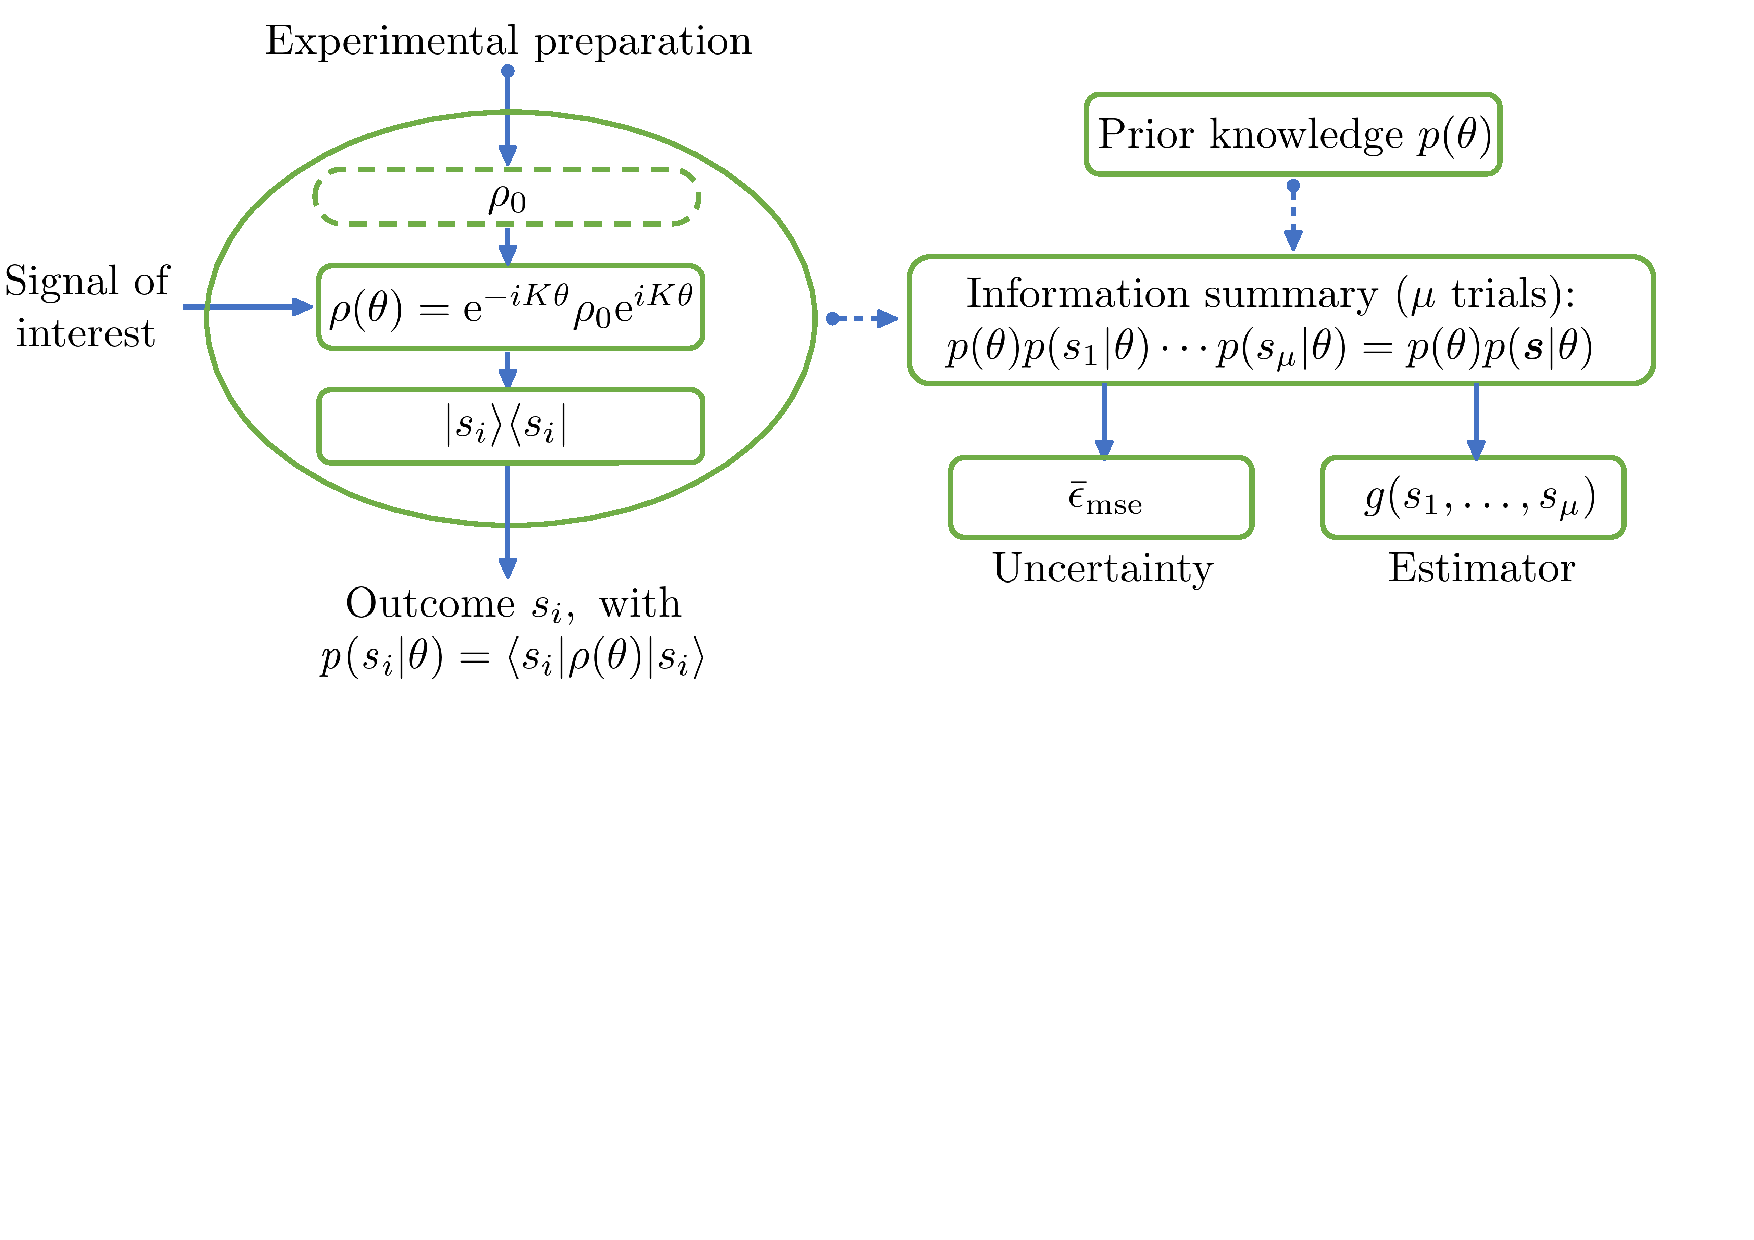
\includegraphics[trim={0.1cm 9.25cm 0.5cm 0cm},clip,width=15cm]{ch5_fig1}
	\caption[Extraction of information from a quantum sensor]{Representation of the extraction of information from a quantum sensor following the shot-by-shot strategy. This process consists of three stages: preparation of the probe state $\rho_0$, parameter encoding $\mathrm{exp}(-i K\theta)$ and measurement scheme $\ketbra{s_i}$. The statistics of the outcome $s_i$ is given by the Born rule, and the protocol is repeated $\mu$ times. Taking also into account any prior information that we may have we can construct an estimator $g(s_1,\dots,s_\mu)$ as a function of the experimental outcomes, and assess its performance using the measure of uncertainty $\bar{\epsilon}_\mathrm{mse}$.}
\label{singleshotvisual}
\end{figure}

\subsection{Calculation scheme for the optimal single-shot strategy}
\label{numcal}

The error in equation (\ref{shotbyshotmse}) can be numerically calculated as a function of $\mu$ following the same three-step algorithm that we discussed in section \ref{subsec:numalgorithm}. On the other hand, to obtain the eigendecomposition of the quantum estimator $S$ that gives rise to the POM $\ketbra{s_i}$ we need to solve $S \rho + \rho S = 2 \bar{\rho}$ for given $\rho_0$, $K$ and $p(\theta)$. 

By expanding $\rho$ in the basis of its eigenvectors, that is, $\rho = \sum_i p_i \ketbra{\phi_i}$, and inserting it into $S \rho + \rho S = 2 \bar{\rho}$, we find that
\begin{equation}
S\rho + \rho S - 2\bar{\rho} = \sum_{ij}\left[\left(p_i + p_j\right)\bra{\phi_i}S\ket{\phi_j} - 2\bra{\phi_i} \bar{\rho} \ket{\phi_j} \right]\ketbra{\phi_i}{\phi_j} = 0,
\end{equation}
so that we can formally express the solution for $S$ as
\begin{equation}
S = 2\sum_{ij} \frac{\bra{\phi_i} \bar{\rho} \ket{\phi_j}}{p_i+p_j}\ketbra{\phi_i}{\phi_j}.
\label{quantumestimator_rho}
\end{equation}
Importantly, equation (\ref{quantumestimator_rho}) is only defined on the support of $\rho$, since $S \rho + \rho S = 2 \bar{\rho}$ is a Sylvester equation and, as such, it only has a unique solution in the subspace where the spectra of $\rho$ and $-\rho$ are disjoint (see pages 203, 204 of \cite{bhatia1997}). However, this is not a problem, since the quantity $\mathrm{Tr}(\bar{\rho}S) = \mathrm{Tr}(\rho S^2)$ appearing in the single-shot bound in equation (\ref{singleshot_bound}) only depends on the terms associated with the support of $\rho$, that is, 
\begin{equation}
\mathrm{Tr}(\rho S^2) = \sum_{i} p_i \bra{\phi_i} S^2 \ket{\phi_i} = \sum\limits_{\substack{\lbrace i,\hspace{0.2em} p_i\neq 0 \rbrace}} p_i \bra{\phi_i} S^2 \ket{\phi_i}.
\end{equation}

Unfortunately, the analytical calculation of equation (\ref{quantumestimator_rho}) is challenging for indefinite photon number states, since they belong to a space whose dimension is infinite. For that reason, we have employed a hybrid method where $\rho$ and $\bar{\rho}$ are calculated analytically and $S$ is obtained numerically from equation (\ref{quantumestimator_rho}) with the algorithm in appendix \ref{sec:singleshotalgorithm}. 

To find the analytical expressions of $\rho$ and $\bar{\rho}$, first we recall that the generator for the Mach-Zehnder interferometer that we are analysing is $K = J_z$. By expanding the transformed pure state $\ket{\psi(\theta)} = \mathrm{e}^{-i J_z\theta}\ket{\psi_0}$ in the number basis as $\ket{\psi(\theta)} = \sum_{nm}\mathrm{e}^{-i (n-m)\theta/2}c_{nm}\ket{nm}$, where $c_{nm}$ are the components of the initial state $\ket{\psi_0}$, we can construct the density matrix
\begin{equation}
\rho(\theta) = \ketbra{\psi(\theta)} =\sum_{nmlk} \mathrm{e}^{-i (n-m)\theta/2} \mathrm{e}^{i (k-l)\theta/2} c_{nm}c^{*}_{kl}\ketbra{nm}{kl},
\end{equation}
with $c_{nm}c_{kl}^{*}=\left(\rho_{0}\right)_{nmkl}$. Then, given that $p(\theta)=1/W_0$ when $\theta$ lies between $\bar{\theta} - W_0/2$ and $\bar{\theta} + W_0/2$, we have that
\begin{equation}
\rho = \int d\theta p(\theta) \rho(\theta)= \sum_{nmkl} \mathcal{K}_{nmkl} c_{nm}c^{*}_{kl}\ketbra{nm}{kl}
\label{zeroth_qmoment_code}
\end{equation}
and
\begin{equation}
\bar{\rho} = \int d\theta p(\theta)\rho(\theta) \theta = \sum_{nmkl} \mathcal{L}_{nmkl} c_{nm}c^{*}_{kl}\ketbra{nm}{kl},
\label{first_qmoment_code}
\end{equation}
where
\begin{equation}
\mathcal{K}_{nmkl} = \frac{1}{W_0}\int_{\bar{\theta}-W_0/2}^{\bar{\theta}+W_0/2}d\theta \mathrm{e}^{-ix_{nmkl}\theta/2},
\label{k_semianalytical_int}
\end{equation}
\begin{equation}
\mathcal{L}_{nmlk} = \frac{1}{W_0}\int_{\bar{\theta}-W_0/2}^{\bar{\theta}+W_0/2} d\theta \theta \mathrm{e}^{-ix_{nmkl}\theta/2}
\end{equation}
and $x_{nmkl}=n-m+l-k$. These integrals can be computed directly, finding that
\begin{equation}
\mathcal{K}_{nmkl} = \frac{4}{W_0}\frac{A_{nmkl} B_{nmkl}}{x_{nmkl}},
\label{k_semianalytical_sol}
\end{equation}
and
\begin{equation}
\mathcal{L}_{nmkl} = \frac{2 A_{nmkl}}{x_{nmkl}} \left(\frac{2 B_{nmkl} D_{nmkl}}{W_0} + iC_{nmkl}\right),
\end{equation}
where we have defined
\begin{align}
A_{nmkl}&=\mathrm{exp}\left(-i x_{nmkl}\bar{\theta}/2\right),
\nonumber \\
B_{nmkl}&=\mathrm{sin}\left(x_{nmkl}W_0/4\right),
\nonumber \\
C_{nmkl}&=\mathrm{cos}\left(x_{nmkl}W_0/4\right)~\mathrm{and}~
\nonumber \\
D_{nmkl}&=\bar{\theta}-2 i/x_{nmkl}.
\label{d_semianalytical_auxiliar}
\end{align}
Note that all the elements $\mathcal{K}_{nmkl}$ and $\mathcal{L}_{nmkl}$ are well defined except when $x_{nmkl}$ vanishes, in which case we have an indetermination. In those cases we need to take the limits
\begin{equation}
\underset{x_{nmlk}\rightarrow 0}{\mathrm{lim}} \mathcal{K}_{nmkl}=1 ,~~\underset{x_{nmkl}\rightarrow 0}{\mathrm{lim}} \mathcal{L}_{nmkl}=\bar{\theta}.
\label{singularcases}
\end{equation}
Since $\mathcal{K}_{nmkl}$, $\mathcal{L}_{nmkl}$ and $c_{nm}c^{*}_{kl}$ can be seen as $(nm \times kl)$ matrices, we can finally rewrite equations (\ref{zeroth_qmoment_code}) and (\ref{first_qmoment_code}) as $\rho = \rho_0 \circ \mathcal{K}$ and $\rho = \rho_0 \circ \mathcal{L}$, where we are using the entrywise product of matrices defined as $X \circ Y = \sum_{ij} X_{ij} Y_{ij}\ketbra{i}{j}$ \cite{horn1985}.

\section{Our methodology in action: results and discussion}
\label{sec:methodlimited}

\subsection{Highly-sensitive states in two-mode interferometry}
\label{employed_states}

Previously we saw that the coherent state $|\alpha/\sqrt{2},-i\alpha/\sqrt{2}\rangle$ is a natural benchmark to evaluate the enhancement derived from quantum resources such as entanglement or squeezing, while the NOON state $(\ket{N,0} + \ket{0,N})/\sqrt{2}$ is an intuitive example of a definite photon number state that reaches the Heisenberg limit \cite{dowling2008} when enough prior knowledge is available (see \cite{berry2012infinite, hall2012} and its analysis in section \ref{subsec:prioranalysis}). This justifies their use in this chapter mainly as a reference, although we will also highlight those features related to the regime of limited data\footnote{Other aspects of these two states have been extensively studied in previous works. See, e.g., \cite{kolodynski2014, jarzyna2016thesis, hall2012, berry2012infinite}.}.

The principal analysis will instead be dedicated to states that are experimentally feasible and whose quantum Fisher information is large with respect to the two previous benchmarks; i.e., we wish to optimise the non-asymptotic regime of states with a great sensitivity. According to the work by Knott \emph{et al.} \cite{PaulProctor2016}, this is precisely the case of the other two probes that we examined in chapter \ref{chap:nonasymptotic}: the twin squeezed vacuum state $\ket{r,r}=S_1(r)S_2(r)\ket{0,0}$, where $S_i(r) = \mathrm{exp}\lbrace[r^{*}a_i^2-r(a_i^{\dagger})^2]/2\rbrace$, and the squeezed entangled state $\mathcal{N}_{ses}\left(\ket{r,0}+\ket{0,r}\right)$, where $\mathcal{N}_{ses} = [2+2/\mathrm{cosh}(|r|)]^{-1/2}$. Additionally, this is also true for the twin squeezed cat state $\mathcal{N}_{tscs}\left[S(r)\left(\ket{\alpha}+\ket{-\alpha}\right)\right]^{\otimes 2}$, with $\mathcal{N}_{tscs}=(2+2\mathrm{exp}(-2|\alpha|^2)^{-1/2}$ and $\ket{\alpha} = D(\alpha)\ket{0}$. 

In order to have a fair comparison, the parameters that define the previous states have been chosen such that, on average, all the strategies utilise the same amount of resources (see the third column in table \ref{tablesummary}). In particular, $\bar{n} = \bra{\psi_0} R \ket{\psi_0} = \bra{\psi_0} (N_1 + N_2) \ket{\psi_0} = 2$ for all $\ket{\psi_0}$. This energy constraint fixes the parameters of all the states except those of the twin squeezed cat state; the parameters of the latter case will be chosen such that the quantum Fisher information is maximum in all the sections of this work except in sections \ref{correlations_section} and \ref{prior_section}, where we also consider an intermediate scenario. Note that the fact that $\bar{n} = 2$ for all our protocols implies that we are working in the low photon number regime \cite{PaulProctor2016}.

\begin{sidewaystable}
\renewcommand{\baselinestretch}{1.0}
\centering
{\renewcommand{\arraystretch}{1.2}
\begin{tabular}{|l|c|c|c|c|c|c|}
\hline
Probe state & $\ket{\psi_0}$  & State parameters  & $\mathcal{Q}$ & $\mathcal{J}$ & $F_q$ & $\mu_{\tau} (\rho)$\\
\hline
\hline
Twin squeezed vacuum state & $S_1(r)S_2(r)\ket{0,0}$ & $r=\mathrm{asinh}\left( 1 \right)$ & $3$ & $0$ & $8$ & $5$ \\ 
\begin{tabular}{@{}l@{}}Twin squeezed cat state (intermediate) \\ Twin squeezed cat state (optimal)\end{tabular} & $\mathcal{N}_{\mathrm{tscs}}\left[S(r)\left(\ket{\alpha}+\ket{-\alpha}\right)\right]^{\otimes 2}$& \begin{tabular}{@{}c@{}}$r=1.103$, $\alpha=1.090$ \\ $r=1.215$, $\alpha=0.9601$\end{tabular} & \begin{tabular}{@{}c@{}}$10.00$ \\ $11.75$\end{tabular}& \begin{tabular}{@{}c@{}}$0$ \\ $0$\end{tabular} & \begin{tabular}{@{}c@{}} $22.00$ \\ $25.49$\end{tabular} & \begin{tabular}{@{}c@{}}$42$ \\ $66$\end{tabular} \\
Squeezed entangled state & $\mathcal{N}_{\mathrm{ses}}\left(\ket{r,0}+\ket{0,r}\right)$ & $r=\log\left(2+\sqrt{3}\right)$ & $9$ & $-0.1$ & $22$ & $45$ \\ 
NOON state & $\left(\ket{N 0}+\ket{0 N}\right)/\sqrt{2}$& $N=2$ &$0$ & $-1$ & $4$ & $116$ \\
Coherent state & $|\alpha/\sqrt{2},-i\alpha/\sqrt{2}\rangle$ & $\alpha = \sqrt{2}$ & $0$ & $0$ & $2$ & $282$ \\ 
\hline
\end{tabular}}
\caption[Properties of several probe states for optical interferometry]{Properties of the probe states considered in the main text. The state parameters have been chosen such that the mean number of photons is $\bar{n} = 2$. Furthermore, $\mathcal{Q}$ and $\mathcal{J}$ represent the amount of intra-mode and inter-mode correlations in the interferometer defined in \cite{sahota2015} and section \ref{subsec:optint}. Finally, $\mu_{\tau}(\rho)$ indicates the state-dependent number of repetitions that are required for the quantum Cram\'{e}r-Rao bound to be a good approximation to the bounds based on the optimal single-shot strategy in figure \ref{bounds_results}, according to the methodology discussed in chapter \ref{chap:nonasymptotic} with relative error $\varepsilon_\tau = 0.05$, prior mean $\bar{\theta}=0$ and prior width $W_0 = \pi/2$. Note that $\rho$ includes the information of the initial probe, the encoding of the signal and the prior knowledge.}
\label{tablesummary}
~\\[15pt]
\centering
{\renewcommand{\arraystretch}{1.2}
\begin{tabular}{|l|c|c|c|c|c|}
\hline
\diagbox{Probe state ~~~~~~~~~~}{$\mu\cdot\bar{\epsilon}_{\mathrm{mse}}(\mu, W_0)$} & $\mu=1$, $W_0=\pi/2$ & $\mu=1$, $W_0=\pi/3$ & $\mu=1$, $W_0=\pi/4$ & $\mu=1$, $W_0=0.1$ & $\mu \gg 1$ \\
\hline
\hline 
Twin squeezed vacuum state & $9.93\cdot 10^{-2}$ & $5.83\cdot 10^{-2}$ & $3.81\cdot 10^{-2}$ & $8.28\cdot 10^{-4}$ & $1.25\cdot 10^{-1}$  \\ 
Twin squeezed cat state (intermediate) & $1.50\cdot 10^{-1}$ & $6.48\cdot 10^{-2}$ & $3.61\cdot 10^{-2}$ & $8.19\cdot 10^{-4}$ & $4.55\cdot 10^{-2}$  \\ 
Twin squeezed cat state (optimal) & $1.42\cdot 10^{-1}$ & $7.10\cdot 10^{-2}$ & $4.11\cdot 10^{-2}$ & $8.17\cdot 10^{-4}$ & $3.92\cdot 10^{-2}$  \\ 
Squeezed entangled state & $1.12\cdot 10^{-1}$ & $5.61\cdot 10^{-2}$ & $3.47\cdot 10^{-2}$ & $8.19\cdot 10^{-4}$ & $4.55\cdot 10^{-2}$   \\ 
NOON state & $1.04\cdot 10^{-1}$ & $6.47\cdot 10^{-2}$ & $4.21\cdot 10^{-2}$ & $8.31\cdot 10^{-4}$ & $2.5\cdot 10^{-1}$  \\
Coherent state & $1.44\cdot 10^{-1}$ & $7.71\cdot 10^{-2}$ & $4.66\cdot 10^{-2}$ & $8.33\cdot 10^{-4}$ & $5\cdot 10^{-1}$   \\ 
\hline
\end{tabular}}
\caption[Local regimes: single-shot with informative prior, and asymptotic]{Optimal single-shot mean square error with different prior widths for the states considered in the main text and asymptotic performance for $\mu\gg1$. The state parameters are those indicated in table \ref{tablesummary}. We notice that the asymptotic ordering of probe states and the ordering for $W_0=0.1$ and a single shot are identical, which implies that the local regime is achieved for such a prior width.}
\label{prior_effect_summary}
\end{sidewaystable}

Finally, we will assume that the prior width is $W_0 = \pi/2 < 2$ and that the prior mean is $\bar{\theta} = 0$. The former is consistent with our findings in chapter \ref{chap:nonasymptotic}, while the latter is justified by the fact that, as we will see, the fundamental bounds generated by the method in section \ref{sec:methodb} do no depend on $\bar{\theta}$, and $\bar{\theta} = 0$ is more natural than $\bar{\theta} = W_0/2$ in optical interferometry \cite{demkowicz2011}. Moreover, the results that arise from $\bar{\theta} = 0$ and those associated with $\bar{\theta} = W_0/2$ can be related with controllable phase shifts as part of the POM. This will be demonstrated in section \ref{measurements_section}.

\subsection{Quantum bounds in the presence of limited data}
\label{main_results}

The application of the method described in section \ref{sec:methodb} to interferometric configurations leads to the results shown in figure \ref{bounds_results}.i, where the mean square error in equation (\ref{shotbyshotmse}) is plotted as a function of the number of repetitions for the optical probes in section \ref{employed_states}: (a) coherent state, (b) NOON state, (c) twin squeezed vacuum state, (d) squeezed entangled state and (e) twin squeezed cat state. Let us proceed to analyse the consequences of these graphs.

To start with, figure \ref{bounds_results}.i presents two different regimes. On the one hand, the performance of all the states becomes linear with the number of repetitions in the logarithmic scale when $\mu \gtrsim 10^2$. This is precisely the behaviour that we would expect in the asymptotic regime $\mu \gg 1$, since in that case the mean square error can be approximated by the Cram\'{e}r-Rao bound as $\bar{\epsilon}_{\mathrm{mse}}\approx 1/(\mu F)$, and as such $\mathrm{log}(\bar{\epsilon}_{\mathrm{mse}}) \approx - \mathrm{log}(\mu) - \mathrm{log}(F)$. In this regime we can observe that the graphs of different states do not intersect each other. This property allows us to identify the twin squeezed cat state as the best asymptotic choice, followed by the squeezed entangled state, the twin squeezed vacuum state, the NOON state and, finally, the coherent state, whose performance is the worst. We notice that this is consistent with the findings in \cite{PaulProctor2016}.

\begin{figure}[t]
\centering
\begin{tabular}{l l}
\begin{tabular}{@{}c@{}}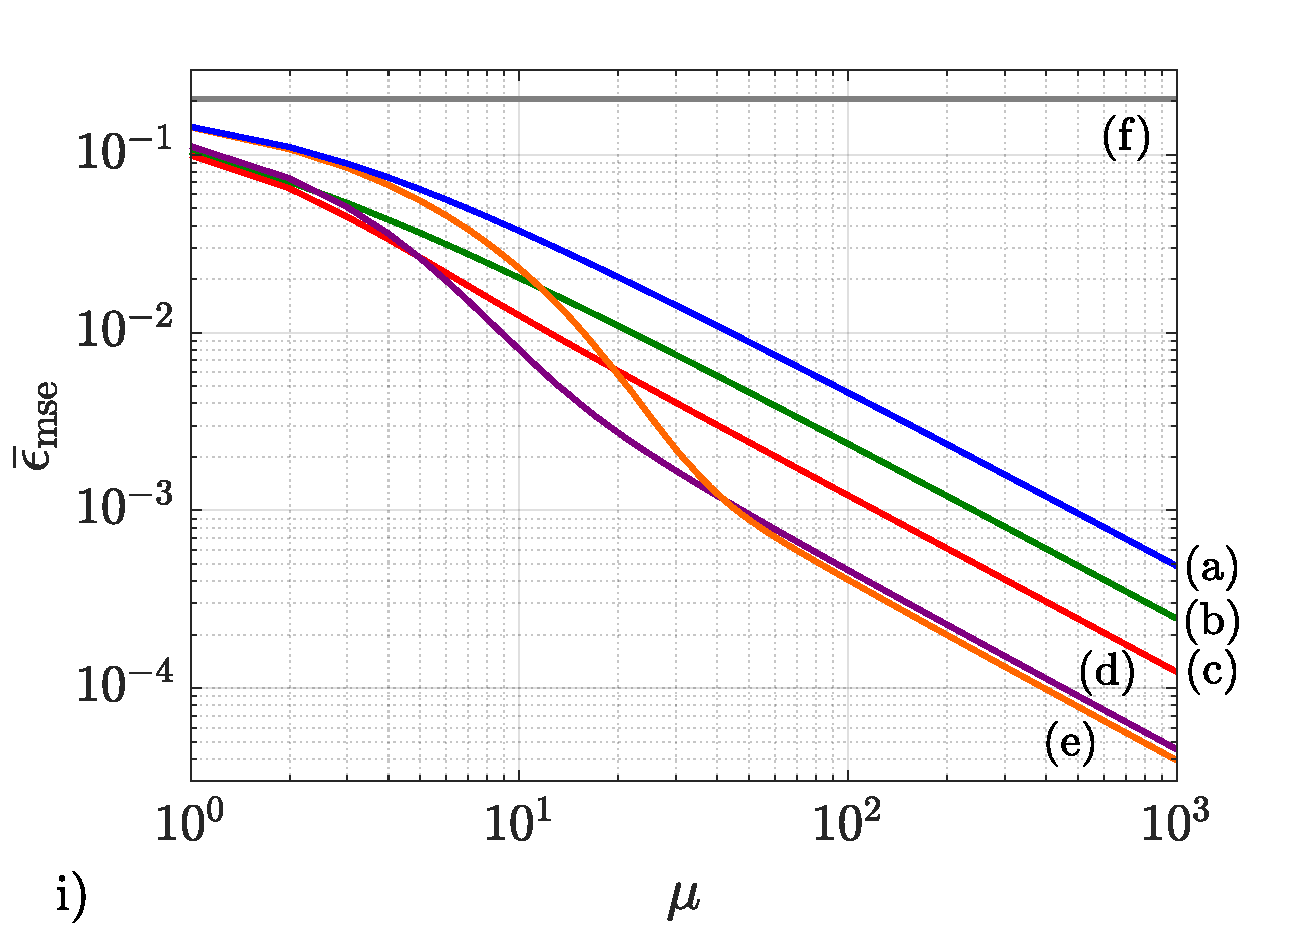
\includegraphics[trim={0.2cm 0.1cm 1cm 1.2cm},clip,width=9.65cm]{ch5_fig2i}\end{tabular} & \begin{tabular}{@{}c@{}} 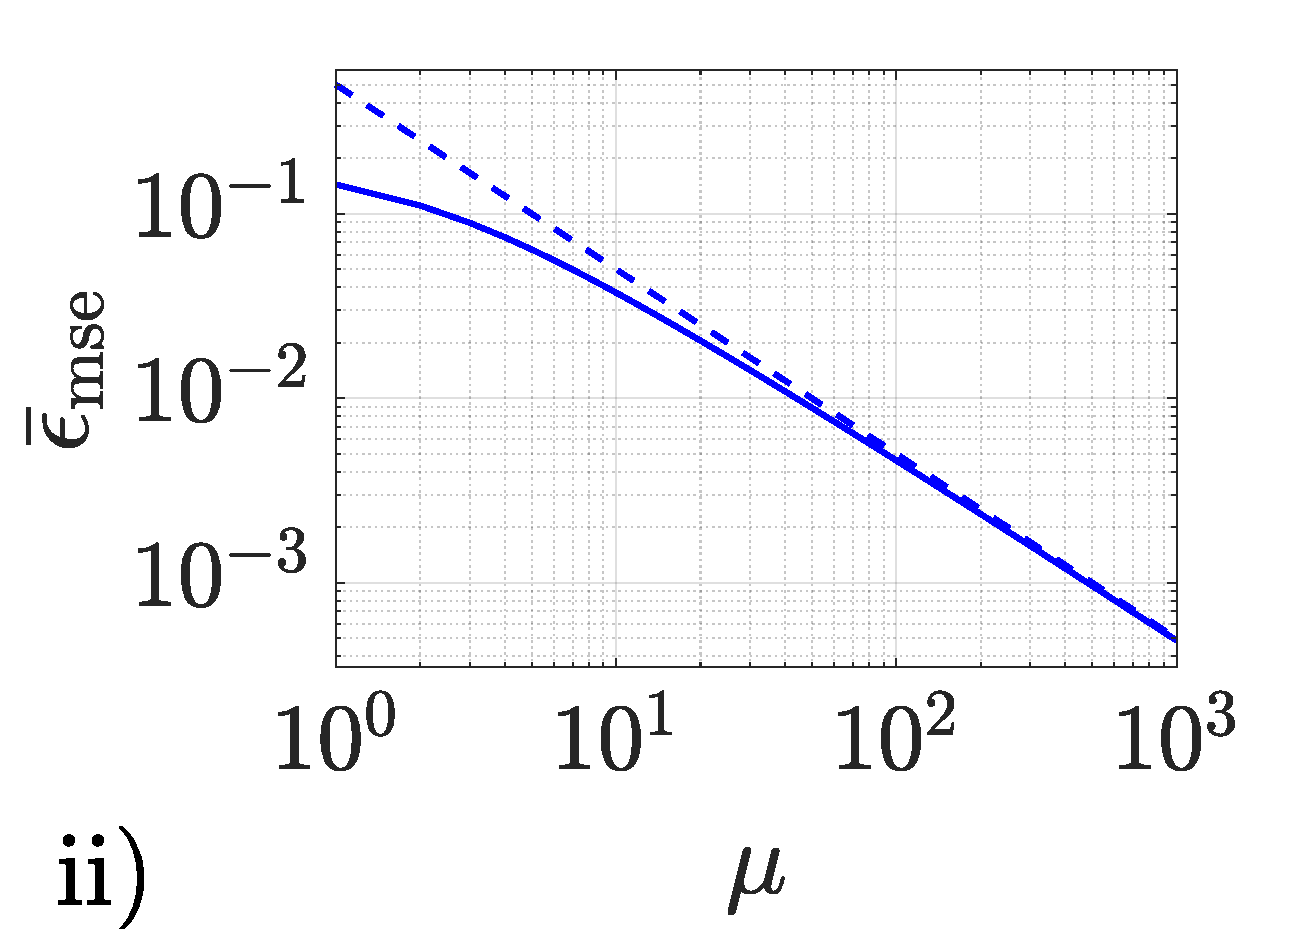
\includegraphics[trim={0.35cm 0cm 1.1cm 1cm},clip,width=4.85cm]{ch5_fig2ii} \\ 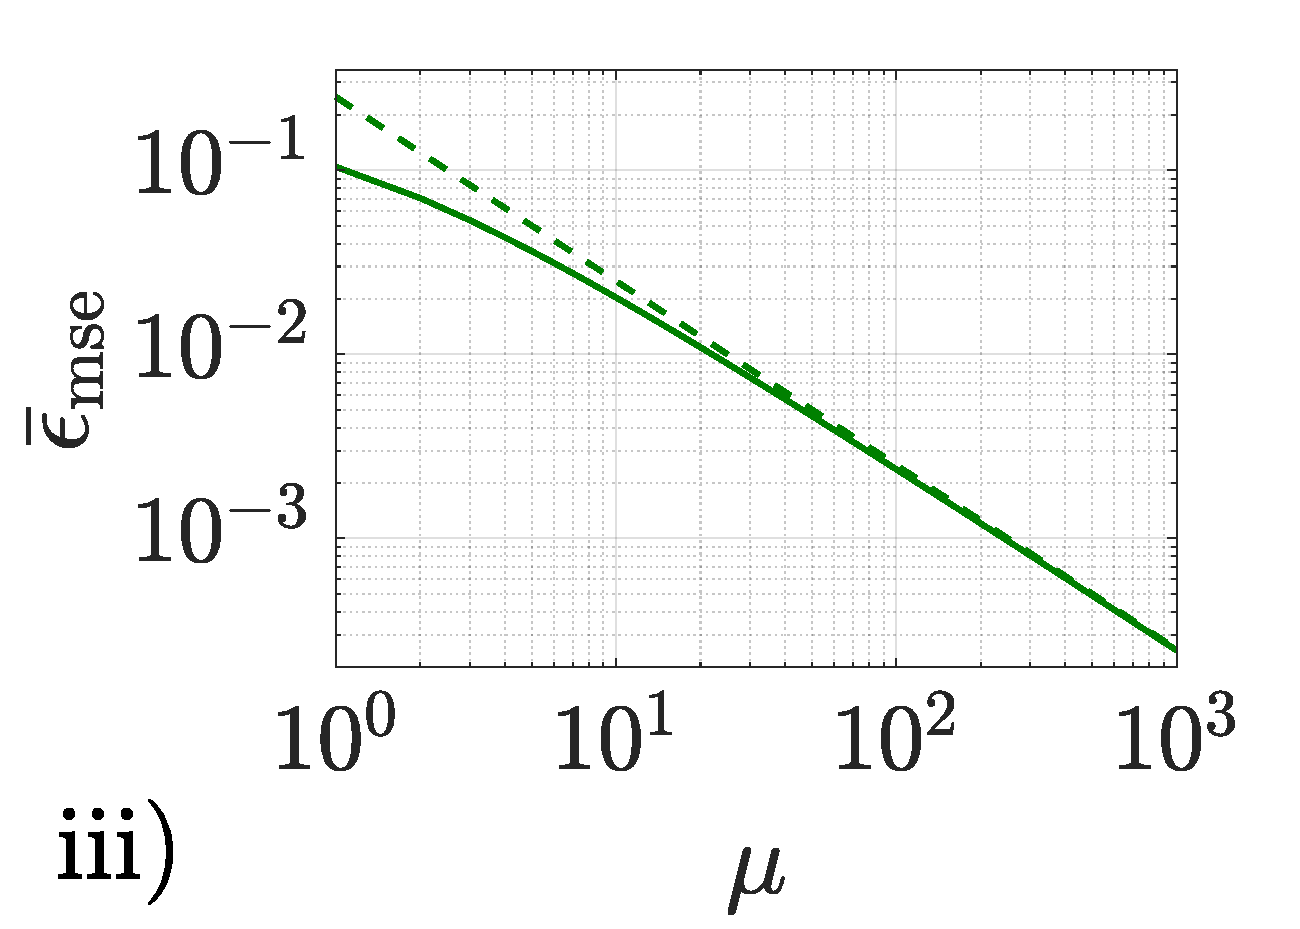
\includegraphics[trim={0.35cm 0cm 1.1cm 1cm},clip,width=4.85cm]{ch5_fig2iii}\end{tabular} \\[0pt]
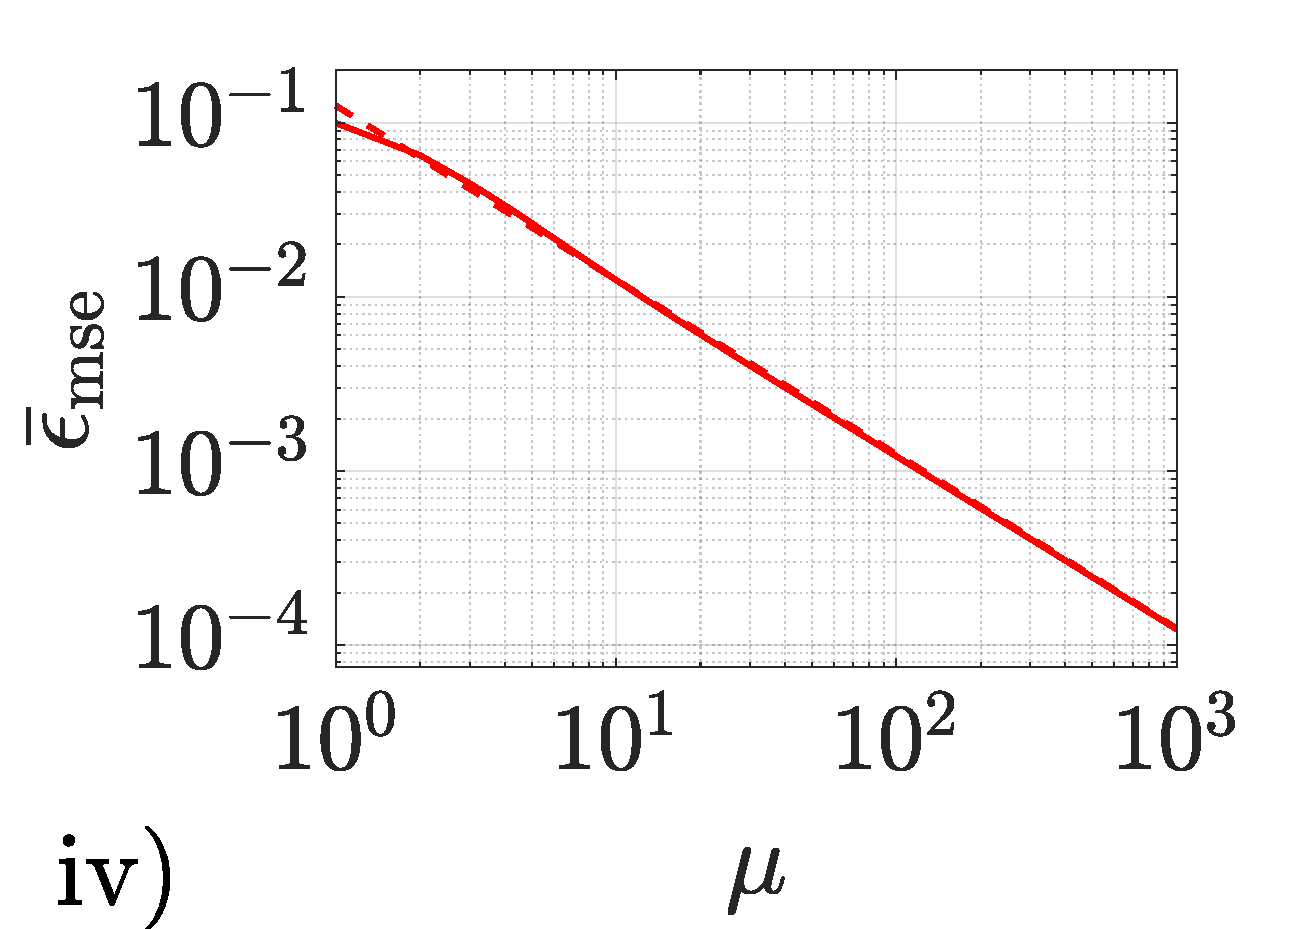
\includegraphics[trim={0.35cm 0cm 1.1cm 1cm},clip,width=4.85cm]{ch5_fig2iv}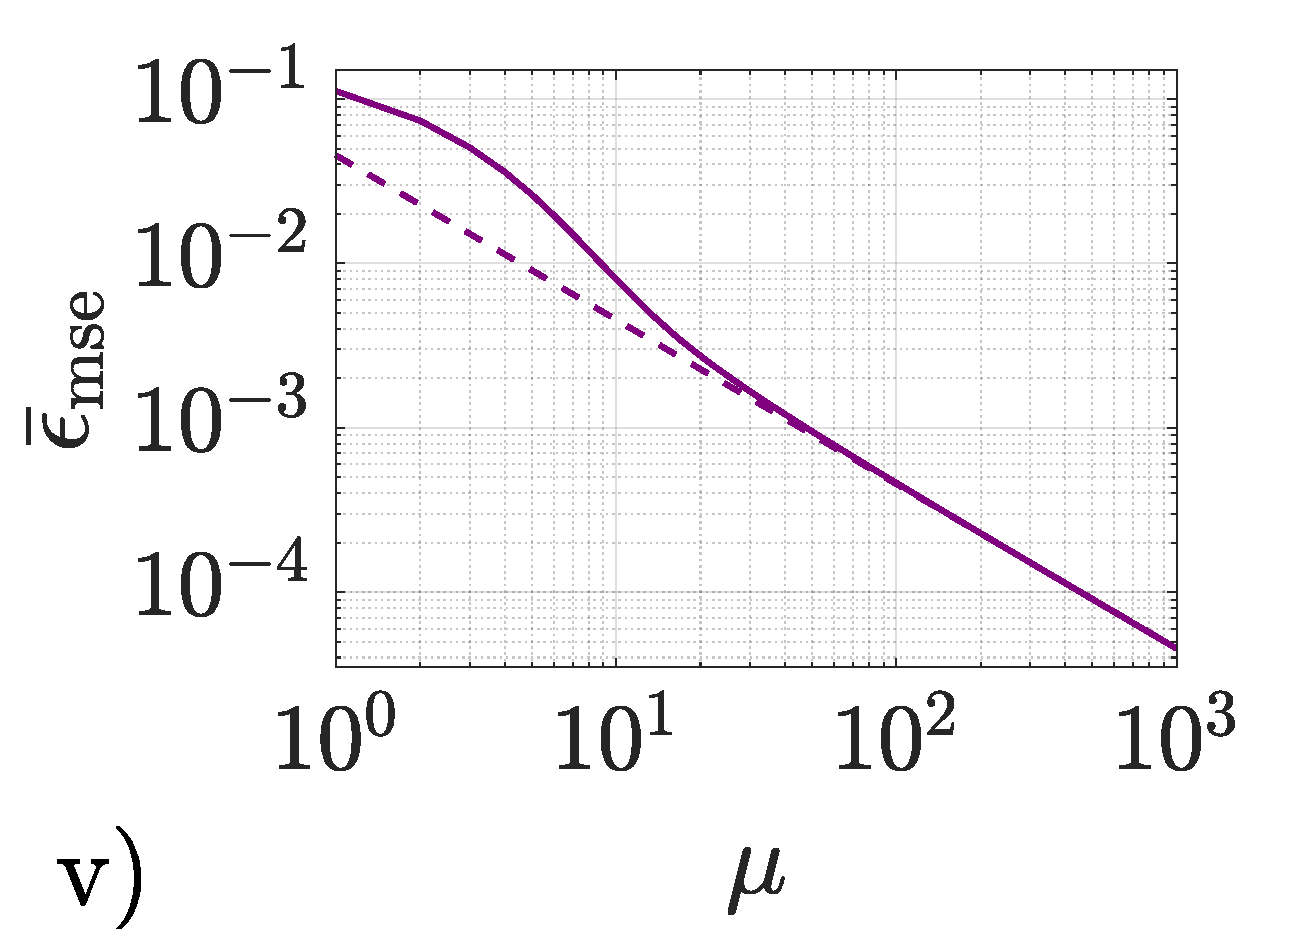
\includegraphics[trim={0.35cm 0cm 1.1cm 1cm},clip,width=4.85cm]{ch5_fig2v} & 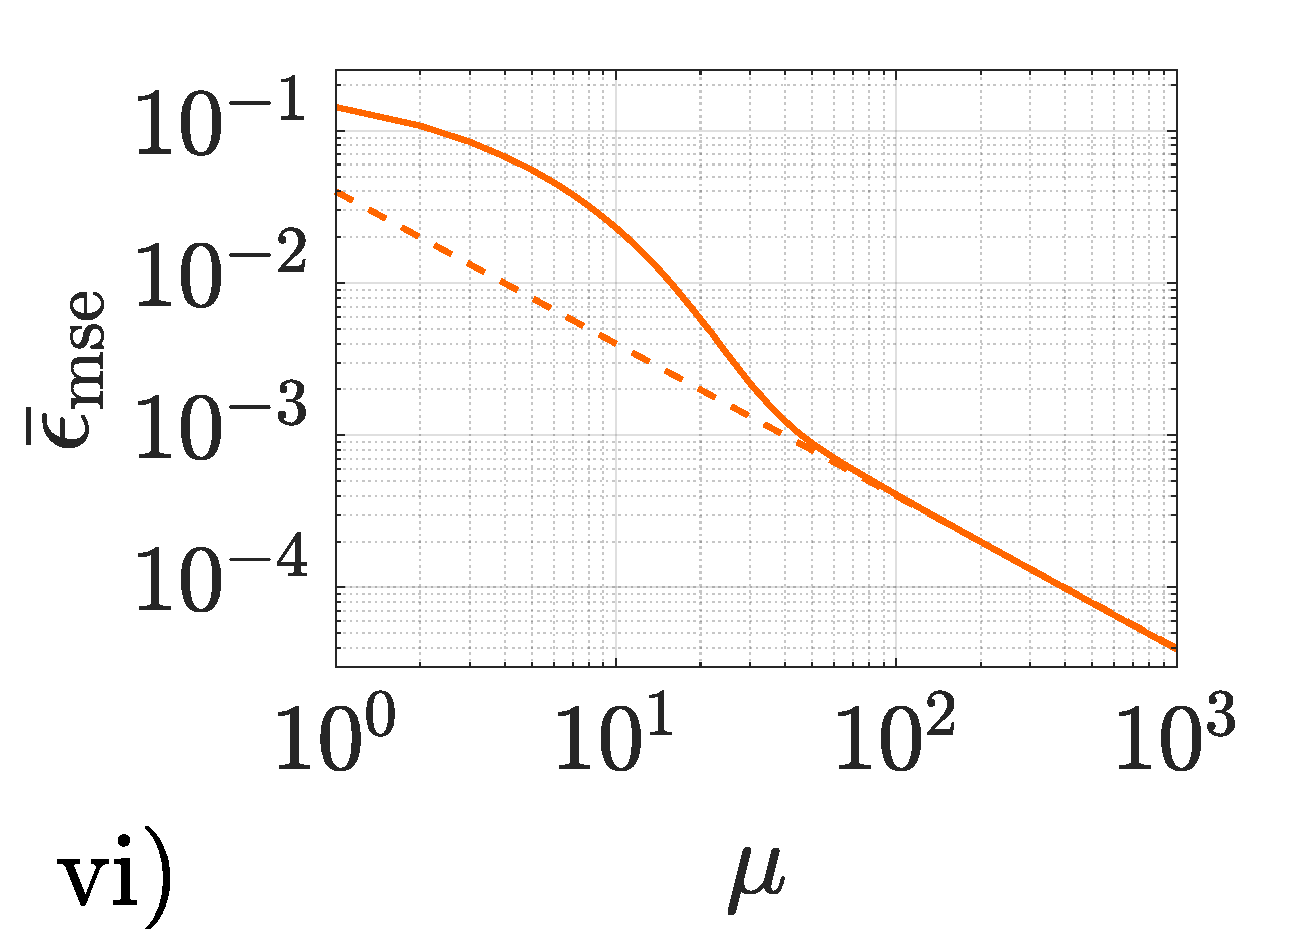
\includegraphics[trim={0.35cm 0cm 1.1cm 1cm},clip,width=4.85cm]{ch5_fig2vi}  \\[0pt]
\end{tabular}
\caption[Shot-by-shot quantum bounds for the Mach-Zehnder interferometer]{i) Mean square error as a function of the number of repetitions using the optimal single-shot strategy for (a) the coherent state, (b) the NOON state, (c) the twin squeezed vacuum state, (d) the squeezed entangled state, and (e) the twin squeezed cat state, with mean number of photons $\bar{n}=2$, prior mean $\bar{\theta} = 0$ and prior width $W_0 = \pi/2$, while (f) represents the variance of the prior probability; (ii) mean square error based on the optimal single-shot strategy (solid line) and quantum Cram\'{e}r-Rao bound (dashed line) for the same coherent state, (iii) NOON state, (iv) twin squeezed vacuum state, (v) squeezed entangled state and (vi) twin squeezed cat state considered in (i). These graphs constitute the main results of section \ref{main_results}, and their consequences are analysed in the main text.}
\label{bounds_results}
\end{figure}

On the other hand, the graphs deviate from this logarithmic linear approximation when $1 \leqslant \mu \lesssim 10^2$ and, as a consequence, a non-trivial structure emerges in this part of the plot. This is the non-asymptotic regime of limited data for the schemes in this chapter. Since the graphs no longer follow straight lines, they intersect each other, and this implies that the ordering of the states in terms of their performance depends on the number of repetitions. For instance, the twin squeezed vacuum state produces the lowest uncertainty when $1\leqslant\mu<5$, while the squeezed entangled state is the best option when $5<\mu<40$. In addition, the twin squeezed cat state is recovered as the best probe when $\mu>40$, although it practically has the same performance as the coherent state when  $\mu = 1, 2 , 3$. Interestingly, the coherent state is also associated with the largest uncertainty for a low number of trials.

That the strategy leading to the lowest uncertainty can depend on the number of repetitions in a crucial way was already demonstrated in chapter \ref{chap:nonasymptotic}. However, our previous results were based on a specific measurement scheme (counting photons after the action of a $50$:$50$ beam splitter), while now the bounds are constructed by repeating a single-shot strategy that has been optimised over all possible POMs. Thus, the results in figure \ref{bounds_results}.i generalise those in chapter \ref{chap:nonasymptotic} and put the state-dependence behaviour of the non-asymptotic regime on a more solid basis.

For these results to be useful, we need to understand the optimality and saturability of the bounds. The uncertainty for $\mu = 1$ is already optimal by construction and can always be reached in principle for any given state using the single-shot POM in equation (\ref{singleshot_strategy}). This means that other tools such as the quantum Ziv-Zakai bound \cite{tsang2012} and the quantum Weiss-Weinstein bound \cite{tsang2016} will necessarily produce less tight single-shot results whenever their value is different from the solution found here. The demonstration of this fact is provided in section \ref{sec:alternativevssingleshot}.

Furthermore, figures \ref{bounds_results}.ii - \ref{bounds_results}.vi show how our results for each state approach the quantum Cram\'{e}r-Rao bound asymptotically, that is, $\bar{\epsilon}_{\mathrm{mse}} \approx 1/(\mu F_q)$  when $\mu \gg 1$. Taking into account that the bounds for a large number of trials that can be constructed using the quantum Cram\'{e}r-Rao bound are fundamental, we conclude that our bounds are also optimal in this limit. As a result, if we work in the regime of intermediate prior knowledge and $\rho(\theta)$ and $p(\theta)$ are given, then the scheme developed in section \ref{sec:methodb} is optimal both for a single shot and a large number of trials. Moreover, it is also optimal for any number of trials if we exclude the possibility of having adaptive measurements and focus on identical and independent experiments.

To quantify the number of repetitions that are needed to reach this asymptotic regime where our methods are no longer required we can follow section \ref{subsec:asymsatu}, construct the relative error $\varepsilon_\tau = |\bar{\epsilon}_{\mathrm{mse}}(\mu_{\tau}) - 1/(\mu_{\tau} F_q)|/\epsilon_{\mathrm{mse}}(\mu_{\tau})$ in equation (\ref{saturation}) and select $\mu_{\tau}$ after imposing that $\varepsilon_\tau \approx 0.05$ for each state. According to the results of this calculation, which are summarised in the last column of table \ref{tablesummary}, the uncertainty for the twin squeezed vacuum state agrees with the prediction of the quantum Cram\'{e}r-Rao bound when the number of trials is as low as $\mu_{\tau} = 5$. Therefore, in this case the asymptotic theory mostly gives the right answer. However, the squeezed entangled state and the twin squeezed cat state require $\mu_{\tau}=45$ and $\mu_{\tau}=66$, respectively, and the quantum Cram\'{e}r-Rao bound overestimates the performance of these probes in the regime of limited data because the graphs of our bounds are higher (figures \ref{bounds_results}.v and \ref{bounds_results}.vi). We note that it is in scenarios of this type where we could not extract useful information from the quantum optimal-bias bound derived in \cite{liu2016}, since for a flat prior this quantity is always lower than the quantum Cram\'{e}r-Rao bound by construction. Finally, the NOON state needs $\mu_{\tau}=116$ and the coherent state requires $\mu_{\tau}=282$, but the Cram\'{e}r-Rao bound prediction underestimates the precision of these protocols when $\mu$ is low. It is interesting to observe that the chosen probes exemplify the three basic behaviours that we could expect to find in the non-asymptotic regime, that is, that the Cram\'{e}r-Rao bound is lower, higher or approximately equal to the Bayesian mean square error.

It is possible to perform the explicit calculation of the optimal measurement scheme that generates the results associated with the NOON state. Using the notation introduced in section \ref{numcal}, its initial density matrix is
\begin{equation}
\rho_0 = 
\begin{pmatrix}
\left(\rho_0\right)_{2020} & \left(\rho_0\right)_{2002} \\
\left(\rho_0\right)_{0220} & \left(\rho_0\right)_{0202}
\end{pmatrix} = \frac{1}{2}
\begin{pmatrix}
1 & 1 \\
1 & 1 \\
\end{pmatrix},
\end{equation} 
while from equations (\ref{k_semianalytical_sol} - \ref{singularcases}) we have that
\begin{equation}
\mathcal{K} = 
\begin{pmatrix}
\mathcal{K}_{2020} & \mathcal{K}_{2002} \\
\mathcal{K}_{0220} & \mathcal{K}_{0202}
\end{pmatrix} = \frac{1}{\pi}
\begin{pmatrix}
\pi & 2 \\
2 & \pi
\end{pmatrix}
\end{equation}
and
\begin{equation}
\mathcal{L} = 
\begin{pmatrix}
\mathcal{L}_{2020} & \mathcal{L}_{2002} \\
\mathcal{L}_{0220} & \mathcal{L}_{0202}
\end{pmatrix} = \frac{i}{\pi}
\begin{pmatrix}
0 & -1 \\
1 & 0  
\end{pmatrix}
\end{equation}
Therefore, 
\begin{equation}
\rho = \rho_0 \circ \mathcal{K} = \frac{1}{2\pi}
\begin{pmatrix}
\pi & 2 \\
2 & \pi
\end{pmatrix} =
\frac{\mathbb{I}}{2} + \frac{\sigma_x}{\pi}
\label{rhonoon}
\end{equation}
and
\begin{equation}
\bar{\rho} = \rho_0 \circ \mathcal{L} = \frac{i}{2\pi}
\begin{pmatrix}
0 & -1 \\
1 & 0
\end{pmatrix} = \frac{\sigma_y}{2\pi}.
\label{rhobarnoon}
\end{equation}
Inserting equations (\ref{rhonoon}) and (\ref{rhobarnoon}) in $S \rho + \rho S = 2 \bar{\rho}$ we find that the equation to be solved is 
\begin{equation}
S + \frac{1}{\pi}\left\lbrace S, \sigma_x \right\rbrace = \frac{\sigma_y}{\pi},
\end{equation}
where $\left\lbrace X, Y \right\rbrace = X Y + Y X$. Recalling that the anticommutator for the Pauli matrices is $\left\lbrace \sigma_i, \sigma_j \right\rbrace = 2\delta_{ij}$, for $i, j, k = x, y, z$, by inspection we conclude that the solution is $S = \sigma_y/\pi$. This implies that the optimal single-shot POM is given by the eigenvectors
\begin{align}
\ket{s_1} &= \frac{1}{\sqrt{2}} 
\begin{pmatrix} 
i  \\
1  
\end{pmatrix} = \frac{1}{\sqrt{2}} (i\ket{2,0}+\ket{0,2}), 
\nonumber \\
\ket{s_2} &= \frac{1}{\sqrt{2}}
\begin{pmatrix} 
1 \\
i 
\end{pmatrix} = \frac{1}{\sqrt{2}} (\ket{2,0}+i\ket{0,2}),
\label{noon_projectors}
\end{align}
and that the Bayesian estimates that the NOON state predicts for $\theta$ are given by the eigenvalues $s_1=-1/\pi$ and $s_2=1/\pi$. In section \ref{measurements_section} we will construct physical measurements that realise these projectors exactly. In addition, it is important to note that, while this spectrum of estimates is discrete and the difference of phase shifts $\theta$ is a continuous variable, Luis and Pe{\v{r}}ina \cite{alfredo1996} showed that this behaviour is not contradictory due to the existence of an ultimate quantum limit to the uncertainty in phase estimation.

\begin{figure}[t]
\centering
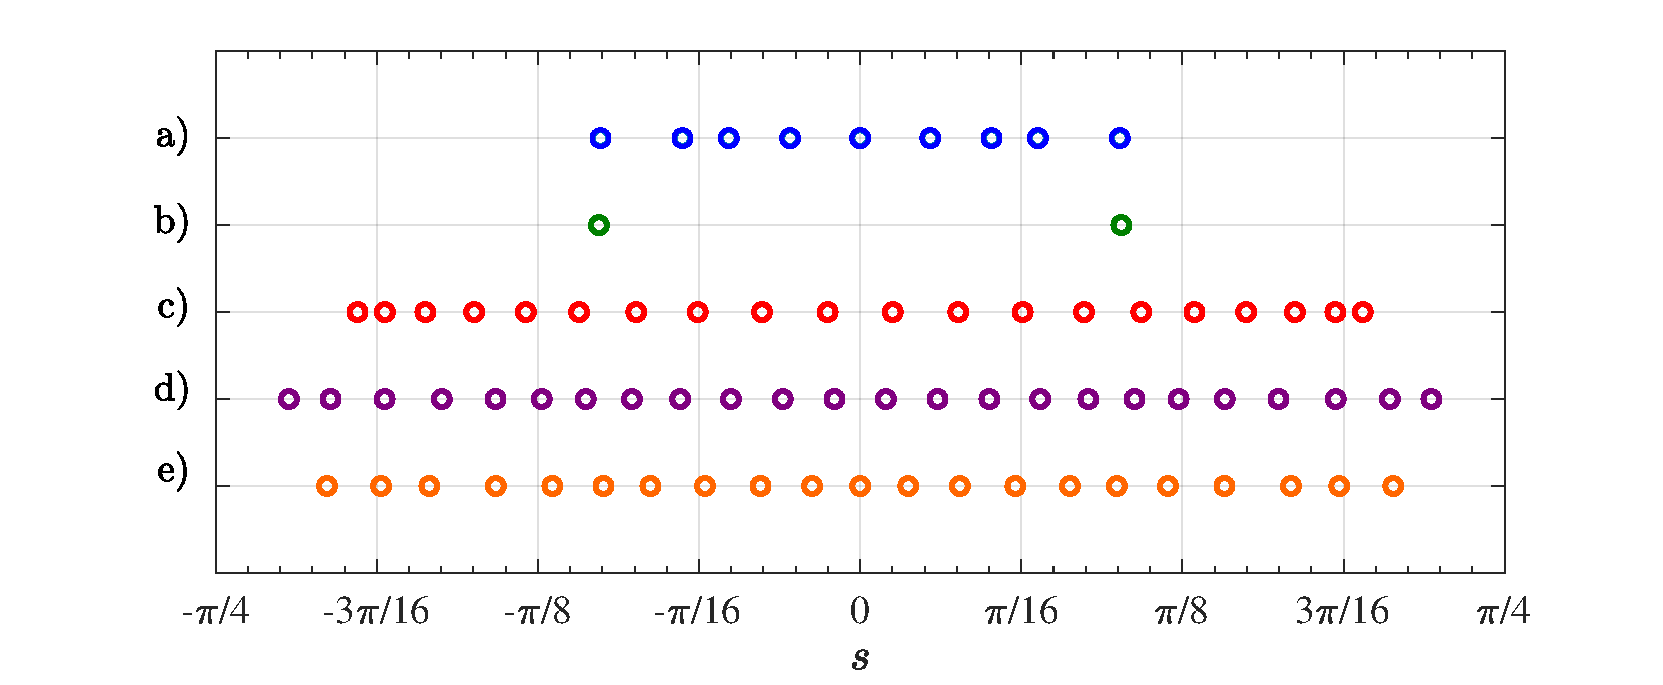
\includegraphics[trim={2.25cm 0.25cm 1.3cm 0.5cm},clip,width=15.5cm]{ch5_fig3}
	\caption[Spectra of the optimal quantum estimators]{Spectrum of the optimal quantum estimator $S$ for (a) the coherent state, (b) the NOON state, (c) the twin squeezed vacuum state, (d) the squeezed entangled state, and (e) the twin squeezed cat state, with $\bar{n}=2$, $\bar{\theta} = 0$ and $W_0 = \pi/2$. The details of this calculation can be found in appendix \ref{sec:singleshotalgorithm}.}
\label{bayes_spectra}
\end{figure}

Although the numerical character of the projectors for the indefinite photon number states makes it difficult to visualise their structure, we can still provide a partial characterisation of these single-shot strategies through the spectra of $S$. A numerical approximation of these spectra has been represented in figure \ref{bayes_spectra} for the coherent state, the twin squeezed vacuum state, the squeezed entangled state and the twin squeezed cat states, which shows their Bayesian estimates distributed within the parameter domain $[\bar{\theta}-W_0/2,\bar{\theta}+W_0/2]$\footnote{We draw attention to the fact that the particular number of estimates represented in the approximated spectra of figure \ref{bayes_spectra} for each indefinite photon number state depends on the numerical truncation of the support where $S$ is defined (see section \ref{numcal}), which in our case assumes that an eigenvalue of $\rho$ is non-zero when its value is higher than $\sim 10^{-12}$. See appendix \ref{sec:singleshotalgorithm} for more details about the numerical approximations employed in this chapter.}.

We finish this analysis by noting that both the projectors $\lbrace \ket{s} \rbrace$ and the estimates $\lbrace s \rbrace$ depend on the specific shape of the prior probability $p(\theta)$. Interestingly, in our case we have verified numerically that while the results change with $W_0$, they do not depend on $\bar{\theta}$. Nonetheless, in section \ref{measurements_section} we will see that this is no longer true for measurement schemes different from the optimal single-shot strategy.

\subsection{The role of intra-mode and inter-mode correlations for a low number of repetitions}\label{correlations_section}

Following our discussion in section \ref{subsec:optint}, there are two types of correlations that are relevant for optical metrology: the intra-mode correlations quantified by the Mandel $\mathcal{Q}$-parameter, and the inter-mode correlations quantified by $\mathcal{J}$. We recall that these quantities were defined in equation (\ref{correlationsintro}) for path-symmetric states, which is the family of probes to which the states in our analysis belong \cite{PaulProctor2016, sahota2015, HofmannHolger2009}. 

These quantities play a crucial role in the regime where $\bar{\epsilon}_{\mathrm{mse}} \approx 1 /(\mu F_q)$ because the quantum Fisher information for path-symmetric pure states can be rewritten as $F_q = 4\Delta J_z^2 = \bar{n}(1+\mathcal{Q})(1-\mathcal{J})$ (\cite{sahota2015, knott2016local} and section \ref{subsec:optint}). Therefore, we can control the asymptotic performance by changing $\mathcal{Q}$ and $\mathcal{J}$. Recalling that $-1\leqslant\mathcal{Q}<\infty$ and $-1\leqslant\mathcal{J}\leqslant 1$, optimising the performance amounts to increasing the intra-mode correlations as much as possible, since path entanglement can only improve the precision by a factor of $2$ at most. To verify that the asymptotic part of figure \ref{bounds_results}.i is consistent with this way of proceeding we have calculated the amount of intra-mode and inter-mode correlations and the quantum Fisher information for each state\footnote{An analytical calculation of these quantities for coherent, NOON and twin squeezed vacuum states is available in \cite{sahota2015} and in section \ref{subsec:commoninter}, while the results for squeezed entangled and twin squeezed cat states can be found in \cite{PaulProctor2016}.}, and the results can be found in the fourth, fifth and sixth columns of table \ref{tablesummary}, respectively. As expected, the twin squeezed cat state, which was found to be the asymptotically optimal choice, has the largest values for $F_q$ and $\mathcal{Q}$ among the states that we are studying.

On the other hand, we have also demonstrated that this state is not better than a coherent state when $\mu \sim 1$, in spite of the fact that for the coherent state we have $\mathcal{Q} = 0$ and $\mathcal{J}=0$, and that the other three probes perform better in the low trial number regime. This already supports the idea that the clear role that photon number correlations play asymptotically is not preserved when $\mu$ is low, something that was suggested by the results in section \ref{subsec:uncertaintynonasymptotic} using a specific POM. While it is not currently possible to find a rigorous relationship between uncertainty and correlations that is also valid in the regime of limited data because an analytical expression for $\bar{\epsilon}_{\mathrm{mse}}(\mu)$ is not available, we can still exploit the methodology introduced in section \ref{sec:methodb} to further explore this idea.

First we note that the twin squeezed cat state can be seen as a family of states defined in terms of the parameters $r$ and $\alpha$. Since this state is separable with respect to the arms of the interferometer, $\mathcal{J} = 0$, and as such we are free to choose different combinations of $r$ and $\alpha$ to control the Mandel $\mathcal{Q}$-parameter while keeping $\bar{n}=2$ and $W_0=\pi/2$ unchanged. The particular instance of the twin squeezed cat family with $\mathcal{Q} = 11.75$ and $F_q = 25.49$ considered until now is the optimal choice after maximising $F_q$ numerically\footnote{The optimisation has been performed using the analytical expression for the quantum Fisher information of the twin squeezed vacuum state that is provided in the appendices of \cite{PaulProctor2016}. Notice that our result is consistent with the equivalent optimisation that was carried out there.}. A second example with $\mathcal{Q} = 10.00$ and $F_q = 22.00$ has been included in table \ref{tablesummary} to represent the intermediate case. In addition, the twin squeezed vacuum state is recovered within the twin squeezed cat family when we choose $\alpha = 0$ \cite{PaulProctor2016}, and for this state we have that $\mathcal{Q} = 3$ and $F_q = 8$. 

\begin{figure}[t]
\centering
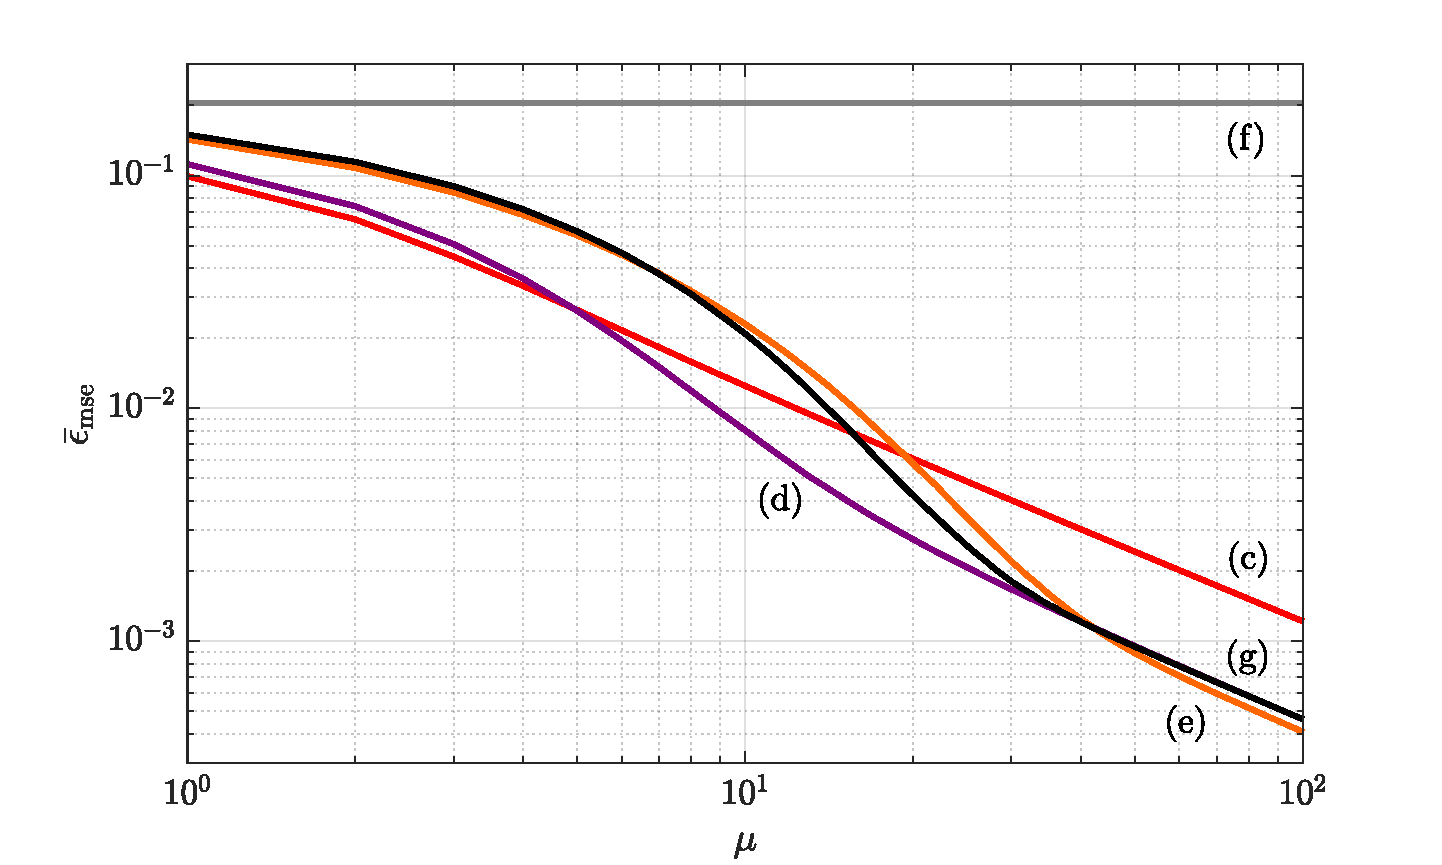
\includegraphics[trim={1cm 0.1cm 1.3cm 1cm},clip,width=14.75cm]{ch5_fig4}
	\caption[Role of photon correlations in the non-asymptotic regime]{Mean square error as a function of the number of repetitions using the optimal single-shot strategy for (c) the twin squeezed vacuum state with $\mathcal{Q}=3$ and $\mathcal{J} = 0$, (d) the squeezed entangled state with $\mathcal{Q}=9$ and $\mathcal{J} = -0.1$, (e) the twin squeezed cat state with $\mathcal{Q}=11.75$ and $\mathcal{J} = 0$, and (e) the twin squeezed cat state with $\mathcal{Q}=10.00$ and $\mathcal{J} = 0$, where $\mathcal{Q}$ and $\mathcal{J}$ quantify the intra-mode and inter-mode correlations, and having $\bar{n}=2$, $\bar{\theta} = 0$ and $W_0 = \pi/2$, while (f) represents the variance of the prior probability.}
\label{correlations_figure}
\end{figure}

Next we examine the mean square errors associated with the optimal case, the intermediate case and the twin squeezed vacuum from the previous family. Their graphs are represented in figure \ref{correlations_figure} and labelled respectively as (e), (g) and (c). If we compare the optimal and intermediate states first, we see that a larger amount of intra-mode correlations is associated with a larger number of repetitions needed to reach the asymptotic regime, since the former state requires $\mu_\tau=66$ and the latter $\mu_\tau=42$ (see table \ref{tablesummary}). Furthermore, by comparing the form of the graphs (e) and (g) in figure \ref{correlations_figure} for these two states we can observe that the transition from the non-asymptotic regime to the asymptotic regime is associated  with a larger uncertainty for the optimal twin squeezed cat state for which $\mathcal{Q}$ is also larger. Finally, the graph (c) shows that the twin squeezed vacuum state, which has the smallest $\mathcal{Q}$, performs worse than the two previous cases asymptotically, while its error is the lowest when $1\leqslant\mu \lesssim 10$. In other words, for this family of states there seems to be a trade-off between the performances in the asymptotic and non-asymptotic regimes that is associated with changes in $\mathcal{Q}$, which in practice would imply that increasing the amount of intra-mode correlations blindly can lead to high-uncertainty schemes in the regime of limited data. Moreover, we note that this conclusion is consistent with the related analysis by Tsang \cite{tsang2012} for the Rivas-Luis state \cite{rivas2012} based on the quantum Ziv-Zakai bound and our own analysis in section \ref{subsec:infiniteprecision}; both approaches demonstrate that if a certain parameter is modified such that the Fisher information increases arbitrarily, then the error cannot deviate substantially from the prior variance unless the number of trials is very large. 

Since increasing $\mathcal{Q}$ seems to be detrimental to the performance of our probes when the number of repetitions is  low, the next natural step is to investigate whether path entanglement could be useful in this regime. Including in our analysis the squeezed entangled state with $\mathcal{Q} = 9$ and $\mathcal{J}=-0.1$, which is labelled as (d) in figure \ref{correlations_figure}, we can see that this state converges asymptotically to the performance associated with the intermediate case of the twin squeezed cat family (g), that is, both probes have the same Fisher information. However, the graph of the squeezed entangled state presents a smaller curvature and a lower uncertainty when $\mu < 30$. The key aspect that distinguishes these two probes is that the squeezed entangled state has a lower amount of intra-mode correlations and a certain amount of beneficial path entanglement, which suggests that inter-mode correlations have helped to improve the precision in the non-asymptotic regime while keeping a large Fisher information. Hence, we conclude that path entanglement could be considerably more relevant in schemes that need to be optimised for a low number of trials than it is in the asymptotic regime. 

Despite these surprising results, we must acknowledge that our analysis is centred on a particular set of states, and that other schemes based on different states could show different properties\footnote{Furthermore, it is reasonable to expect that other schemes that allow other types of correlations behave differently too. For instance, in \cite{smirne2018} the authors showed that allowing entanglement between a finite number of probes in a frequency estimation protocol can lead to a less precise strategy.}. Therefore, the existence of a more general relationship between the number of trials and the usefulness of photon number correlations in interferometry for a given prior is an open question. 

\subsection{The effect of the prior information}
\label{prior_section}

In a wide set of inference problems that includes the scenarios presented here, the importance of the prior information depends on the number of shots. In particular, we know that the prior becomes less important as we increase the number of repetitions \cite{cox2000}, and this implies that, as we argued in chapter \ref{chap:methodology}, the prior probability will play an important role for making inferences if only a few experimental shots are possible. In that scenario it is crucial then to establish how different states of prior knowledge may affect the overall performance of a given metrology scheme.

\begin{figure}[t]
\centering
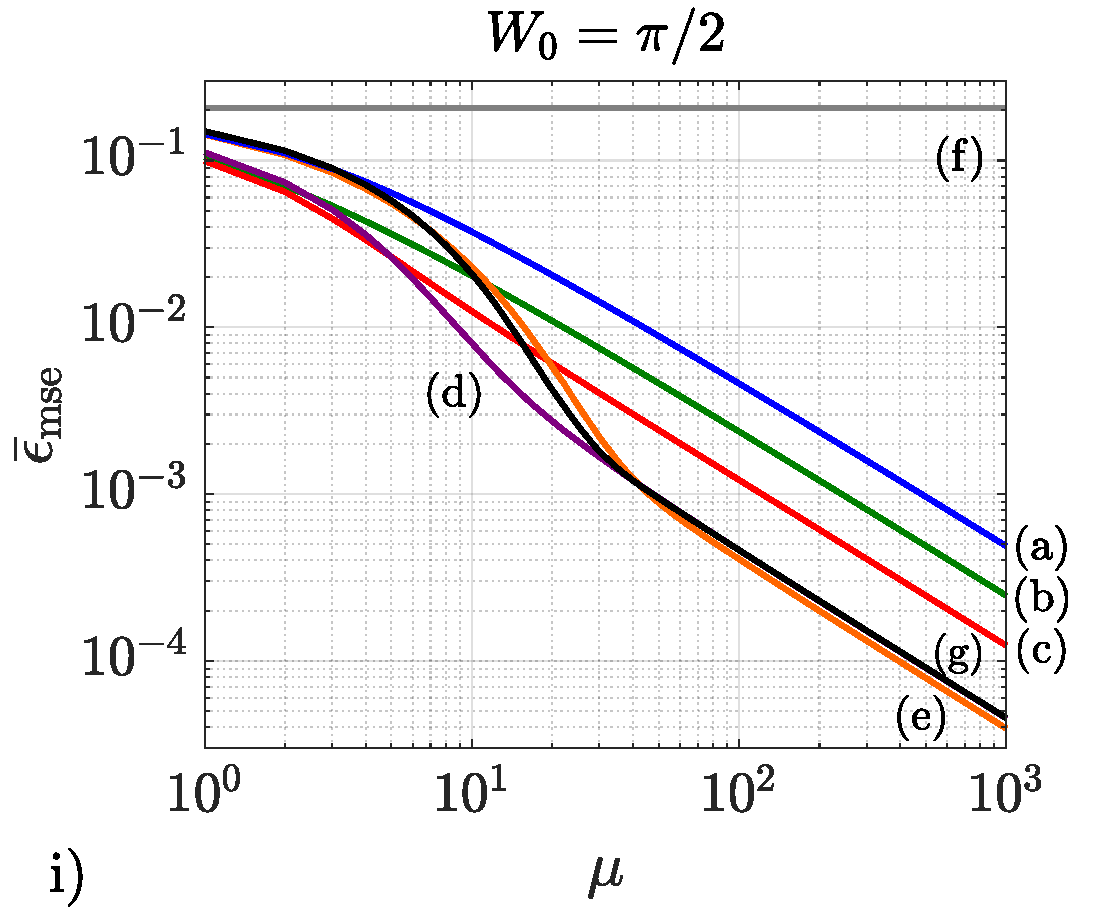
\includegraphics[trim={0.1cm 0.1cm 0.65cm 0.2cm},clip,width=7.7cm]{ch5_fig5i}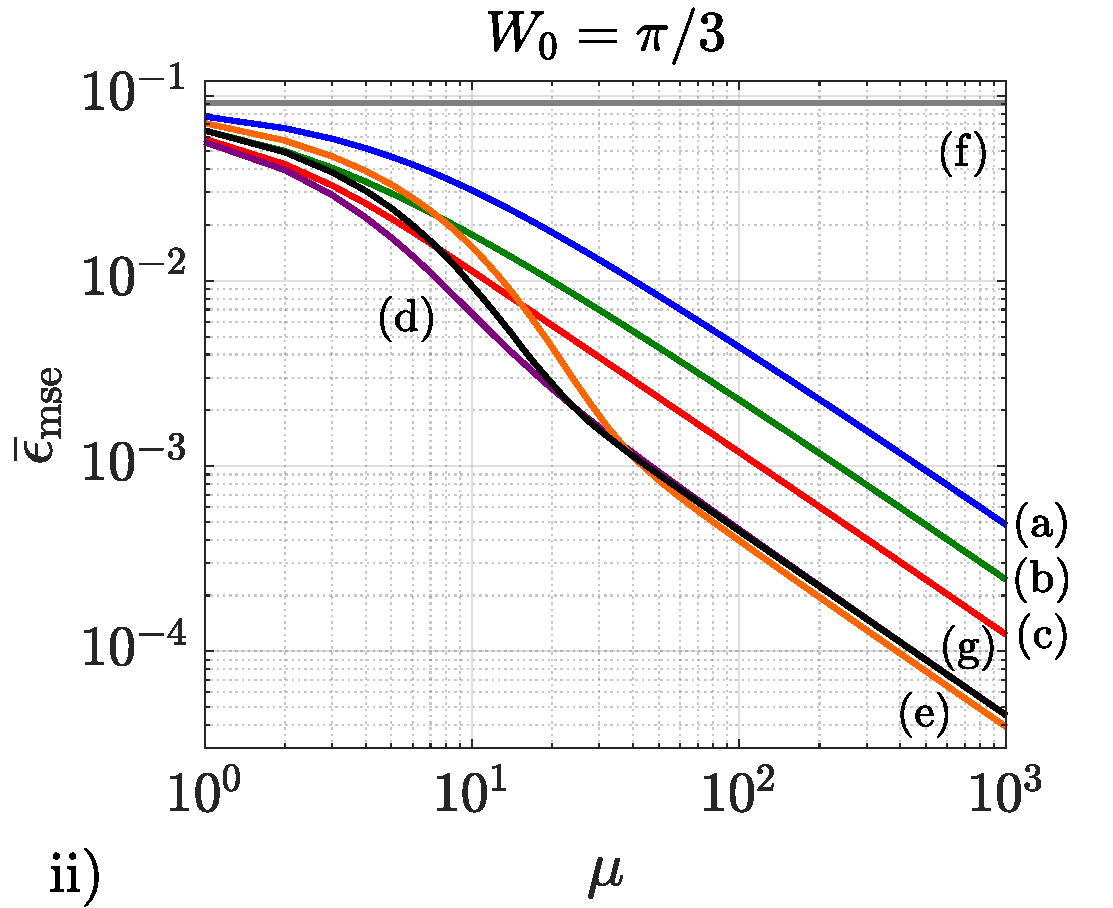
\includegraphics[trim={0.1cm 0.1cm 0.65cm 0.2cm},clip,width=7.7cm]{ch5_fig5ii}
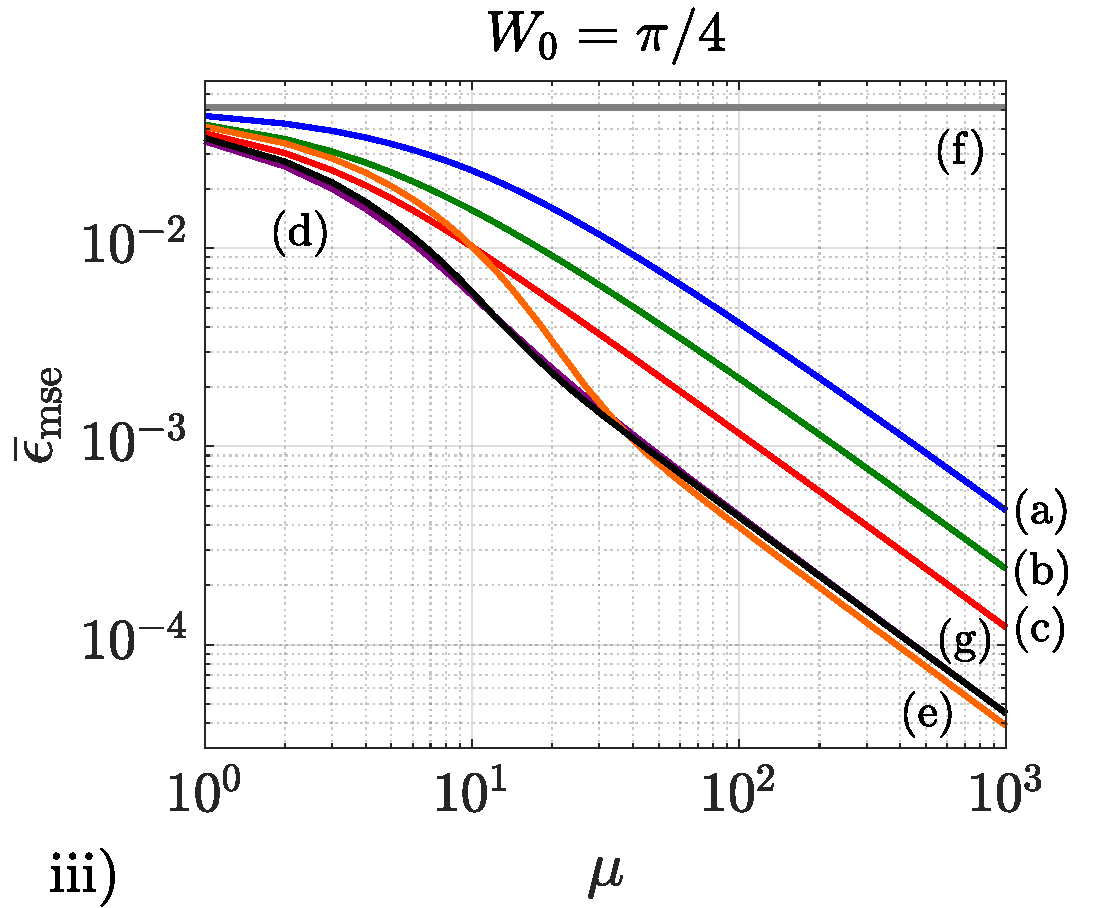
\includegraphics[trim={0.1cm 0.1cm 0.65cm 0cm},clip,width=7.7cm]{ch5_fig5iii}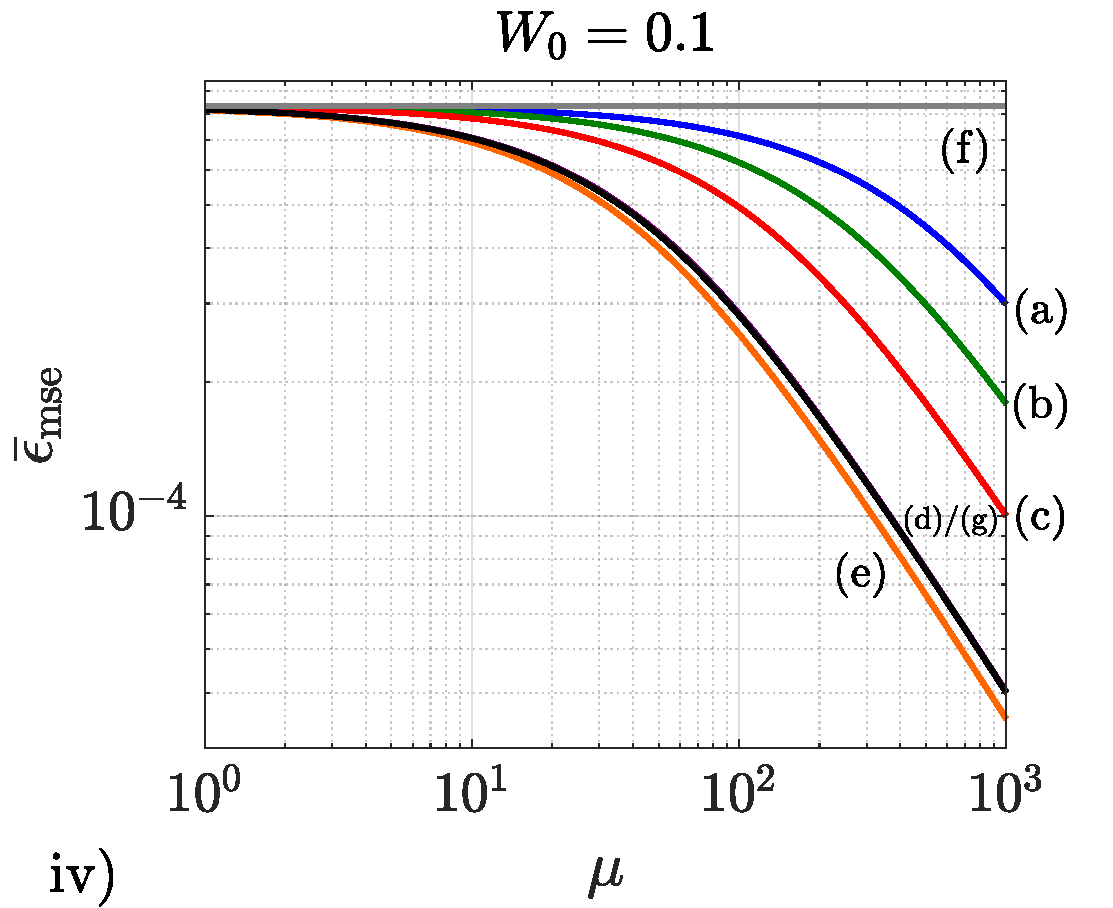
\includegraphics[trim={0.1cm 0.1cm 0.65cm 0.2cm},clip,width=7.7cm]{ch5_fig5iv}
	\caption[Prior information and the transition between local regimes]{i) Mean square error as a function of the number of repetitions using the optimal single-shot strategy for (a) the coherent state, (b) the NOON state, (c) the twin squeezed vacuum state, (d) the squeezed entangled state, (e) the (optimal) twin squeezed cat state, and (g) the (intermediate) twin squeezed cat state, with mean number of photons $\bar{n}=2$, prior mean $\bar{\theta} = 0$ and prior width $W_0 = \pi/2$, while (f) represents the variance of the prior probability; (ii) repetition of the calculation performed in (i) with prior width $W_0=\pi/3$, (iii) $W_0=\pi/4$, and (iv) $W_0=0.1$. The results in these figures represent the transition from the regime of intermediate prior knowledge and a low number of trials to the local regime of a narrow prior and a large number of measurements.}
\label{prior_figure}
\end{figure}

Taking the form of the uniform prior given in equation (\ref{prior_probability}), the parameters that we can alter are the prior width $W_0$ and the prior mean $\bar{\theta}$. In section \ref{main_results} we already mentioned that the bounds constructed in figure \ref{bounds_results}.i do not depend on $\bar{\theta}$, leaving $W_0$ as the only free parameter. In principle we should consider the possibility of having both $W_0>\pi/2$, which includes the intermediate and global regimes, and $W_0<\pi/2$, which encompasses the intermediate and local regimes. However, for large values of $W_0$ it is not possible to approximate the periodic deviation function in equation (\ref{sinerror}) to the square error. For that reason, we will only focus on the transition from the intermediate regime of prior knowledge to the local regime. 

To do this, let us start by calculating the optimal single-shot mean square error (equation (\ref{singleshot_bound}) or equation (\ref{shotbyshotmse}) with $\mu = 1$) for all the states with the prior widths $W_0 = \pi/2,~\pi/3,~\pi/4$ and $0.1$. The numerical results are shown in table \ref{prior_effect_summary}. While the best probe in the single-shot regime for $W_0 = \pi/2$ is the twin squeezed vacuum state, the squeezed entangled state becomes the preferable choice when $W_0 = \pi/3$ and $W_0 = \pi/4$, and we need to start with a prior with width $W_0 = 0.1$ in order to recover the twin squeezed cat state as the optimal state. Moreover, the ordering of probes in terms of their performance when $W_0 = 0.1$ is exactly the same as the ordering found in the asymptotic regime, which is also included in the last column of table \ref{prior_effect_summary}. Consequently, we can say that for our schemes the local regime due to a high amount of prior information is achieved when $W_0 \leqslant 0.1$.

An equivalent path to arrive to the same result relies on the approximation
\begin{equation}
\bar{\epsilon}_{\mathrm{mse}}\gtrsim\Delta \theta_p^2\left(1-\Delta\theta_p^2 F_q\right)
\label{bayes_bound_high_prior}
\end{equation}
employed in \cite{macieszczak2014bayesian, jarzyna2015true} for the single-shot mean square error. This relation was found in \cite{macieszczak2014bayesian} assuming a Gaussian prior with a narrow width but, in fact, it can be shown that it also holds for our flat prior if $W_0 \ll 1$. Assuming the latter condition, the Taylor expansion around $\bar{\theta}$ for the transformed state $\rho(\theta)$ is
\begin{equation} 
\rho(\theta) \approx \rho(\bar{\theta}) + \frac{\partial \rho(\bar{\theta})}{\partial \theta} (\theta - \bar{\theta}).
\label{rhoparameterapprox}
\end{equation}
Furthermore, recalling that $L(\bar{\theta})\rho(\bar{\theta}) + \rho(\bar{\theta}) L(\bar{\theta}) = 2\partial \rho(\bar{\theta})/\partial \theta$ for the symmetric logarithmic derivative $L(\bar{\theta})$ \cite{helstrom1976,paris2009,rafal2015}, equation (\ref{rhoparameterapprox}) can be rewritten as
\begin{equation}
\rho(\theta)  \approx \rho(\bar{\theta}) + \frac{1}{2}\left[ L(\bar{\theta})\rho(\bar{\theta}) + \rho(\bar{\theta}) L(\bar{\theta})\right] (\theta - \bar{\theta} ).
\label{density_matrix_approx}
\end{equation}
The next step is to introduce equation (\ref{density_matrix_approx}) in the expressions $\rho = \int d\theta p(\theta) \rho(\theta)$ and $\bar{\rho} = \int d\theta p(\theta) \rho(\theta) \theta$, finding that $\rho \approx \rho(\bar{\theta})$ and
\begin{equation}
\bar{\rho} \approx \bar{\theta}\rho(\bar{\theta}) +  \frac{\Delta \theta^2_p}{2}\left[ L(\bar{\theta})\rho(\bar{\theta}) + \rho(\theta) L(\bar{\theta})\right].
\end{equation}
Hence, from $S\rho + \rho S = 2\bar{\rho}$ and the previous approximations we can see that the equation to be solved in this regime is
\begin{equation}
\left[S - \theta \mathbb{I} - \Delta \theta^2_p L(\bar{\theta})\right]\rho(\bar{\theta}) + \rho(\bar{\theta}) \left[S - \theta \mathbb{I} - \Delta \theta^2_p L(\bar{\theta})\right] \approx 0, 
\end{equation} 
which means that the quantum estimator takes the form 
\begin{equation}
S \approx \bar{\theta} ~\mathbb{I} + \Delta \theta^2_p ~ L(\bar{\theta}).
\end{equation}
In turn, this implies that 
\begin{equation}
\mathrm{Tr}\left(\bar{\rho}S\right) \approx \bar{\theta}^2 + \Delta \theta^4_p~F_q(\bar{\theta}),
\label{approxbayesinfo}
\end{equation}
where $F_q(\bar{\theta}) = \mathrm{Tr}[\rho(\bar{\theta})L(\bar{\theta})^2]$ and we have used the fact that $\mathrm{Tr}[\rho(\bar{\theta})L(\bar{\theta})] = 0$, and by introducing equation (\ref{approxbayesinfo}) in the single-shot bound $\bar{\epsilon}_{\mathrm{mse}} \geqslant \int d\theta p(\theta)\theta^2 - \mathrm{Tr}(\bar{\rho}S) = \Delta\theta^2_p + \bar{\theta}^2 - \mathrm{Tr}(\bar{\rho}S)$ that was reviewed in sections \ref{subsec:singleshotparadigm} and \ref{subsec:originalderivation} we finally arrive at equation (\ref{bayes_bound_high_prior}).

That the Fisher information $F_q$ appears in equation (\ref{bayes_bound_high_prior}) as the key quantity to determine which scheme has the best performance for a given prior explains why the numerical results in table \ref{prior_effect_summary} for $W_0=0.1$ predict the same order of probes as the approximation $1/(\mu F_q)$ in the asymptotic regime of many repetitions. In both cases, the larger $F_q$, the better the performance. 

It is interesting to observe the similarity between the local regime of prior knowledge for a single shot and the local regime due to a large number of experiments. On the one hand, the best states for $W_0=\pi/2$ and $W_0=0.1$ have intra-mode correlations only, while for $W_0 = \pi/3$ and $W_0 = \pi/4$ the best state presents path entanglement too. On the other hand, figure \ref{prior_figure}.i shows that for $1\leqslant\mu<5$ and $\mu>40$ there is no inter-mode entanglement in the optimal probes, but it appears in the best state for $5<\mu<40$. One way of understanding this similar behaviour is to note that updating our posterior density via Bayes theorem after each new trial reduces the uncertainty in a way that is formally similar to making the prior narrower in a sequential way. Nevertheless, both processes are conceptually different. 

Finally, figures \ref{prior_figure}.i - \ref{prior_figure}.iv show the transition from the intermediate regime of prior knowledge and a low number of trials to a local regime with both high prior information and a large number of shots. This modifies the connection between the number of repetitions and the properties of different probes considerably, as can be seen by the change in the points where the graphs for different states cross each other as the prior width is reduced. As a result, establishing a pattern that helps us to understand what probes we need to use for different values of $\mu$ in the regime of limited data becomes more complicated than in the two previous sections. Fortunately, this is not a problem in real experiments because we typically know what our specific prior information is and we can always proceed on a case-by-case basis, but it constitutes an important obstacle to deriving more general conclusions.

\subsection{Performance of physical measurements}
\label{measurements_section}

Until now we have investigated the physical consequences of the bounds constructed following the procedure of section \ref{sec:methodb}. Nevertheless, in a real-world situation we also need to be able to generate concrete sequences of operations that can be implemented in the laboratory, study whether they saturate the theoretical bounds and, if they do not, determine how close to the fundamental minimum the associated uncertainty is. Since here we are using a fixed set of probe states, we need only consider sequences for implementing the measurement scheme.

States that can be generated using operations such as squeezing or displacement from the vacuum are generally easier to prepare than the abstract (and possibly entangled) states that arise in theoretical optimisations \cite{rafal2015,PaulProctor2016,schafermeier2018}; consequently, there is an intrinsically practical interest in exploring how close to the fundamental bounds this type of state can get. We already know that we can approach the quantum Cram\'{e}r-Rao bound  asymptotically for path-symmetric pure (but otherwise general) states when each individual measurement consists of counting photons after the action of a $50$:$50$ beam splitter \cite{HofmannHolger2009}. For instance, using that POM we have shown in section \ref{subsec:uncertaintynonasymptotic} that if $W_0 = \pi/2$ and we impose that the relative error in equation (\ref{saturation}) is $\varepsilon_{\tau}=0.05$, then this is true for the twin squeezed vacuum state for $\mu_\tau \geqslant 874$, although surpassing the $0.05$ threshold with the squeezed entangled state requires more than $\mu = 10^3$ repetitions because its convergence is slower.

By using the bounds with $W_0=\pi/2$ and $\bar{\theta} = 0$ in section \ref{main_results} we can now answer this question in the regime of limited data too, both for the previous states and for the coherent and the twin squeezed cat states. As a preliminary step we have reproduced these bounds as shaded areas in figures \ref{continuousPOM}.i - \ref{continuousPOM}.iv for the coherent state, the twin squeezed vacuum state, the squeezed entangled state and the twin squeezed cat state, respectively. In addition, the dashed lines in those figures represent the mean square error associated with the measurement of the energy at each port of the interferometer (i.e., counting photons) after the action of a $50$:$50$ beam splitter. We draw attention to the fact that we have also introduced a known phase shift in the second port of the interferometer before this beam splitter is applied, the complete sequence of operations for each state being presented in table \ref{POM_summary}. The reason behind this choice is that we have found that the uncertainty of this POM depends on $\bar{\theta}$, and the extra phase shift allows us to achieve the optimal single shot precision when the prior is centred around $\bar{\theta} = 0$, which is our case. This dependence with $\bar{\theta}$ can be seen as a Bayesian analogue of those cases where the standard error propagation formula for a given observable depends on the unknown parameter $\theta$, which is not a problem in practice provided that the experiment is arranged close to an optimal operating point \cite{rafal2015}.

Importantly, the results in chapter \ref{chap:nonasymptotic} for $W_0=\pi/2$ were based on a prior centred around $\pi/4$ and did not include the extra phase shift discussed in the previous paragraph as part of the measurement scheme. However, we have found that the configuration in chapter \ref{chap:nonasymptotic} generates uncertainties that are numerically similar to those discussed here when the extra phase shifts are taken into account. Therefore, the comparison between both collections of results is meaningful for $W_0=\pi/2$.

\begin{figure}[t]
\centering
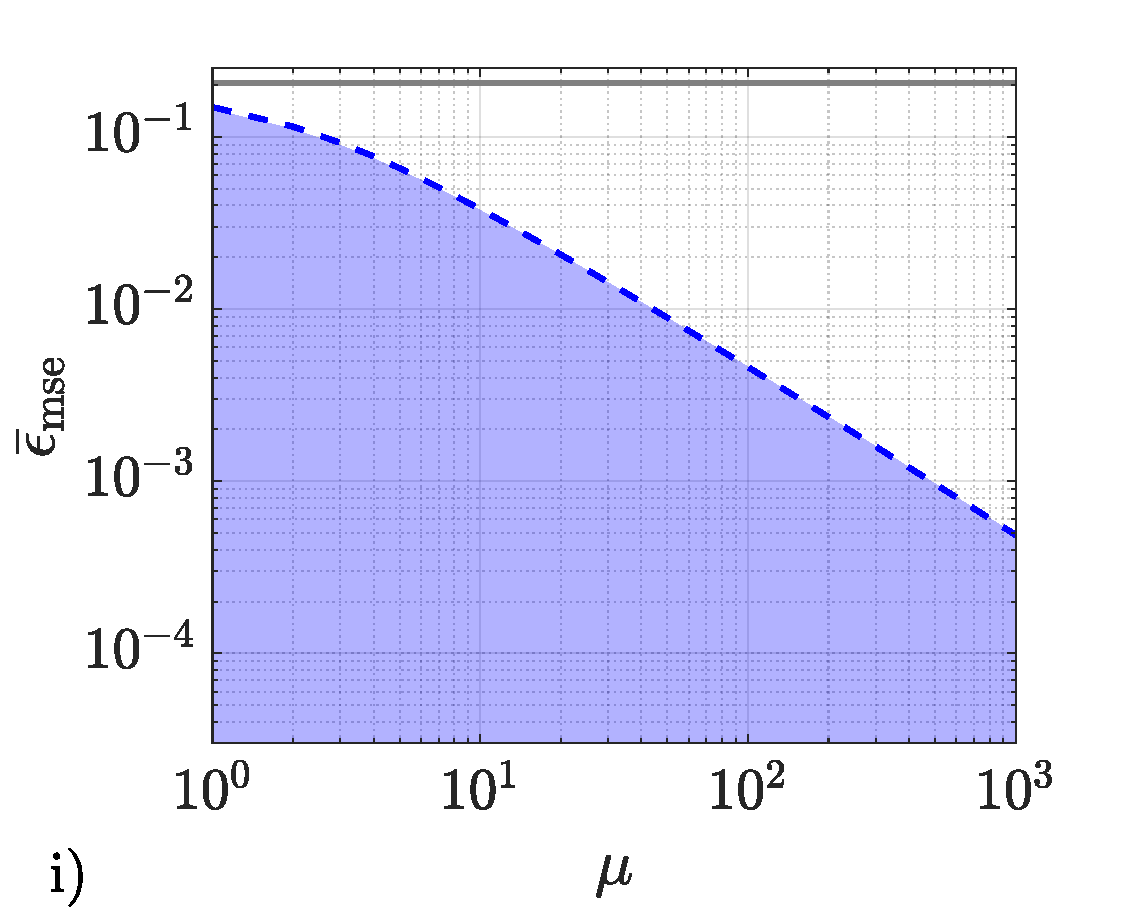
\includegraphics[trim={0.1cm 0.1cm 0.65cm 0.2cm},clip,width=7.7cm]{ch5_fig6i}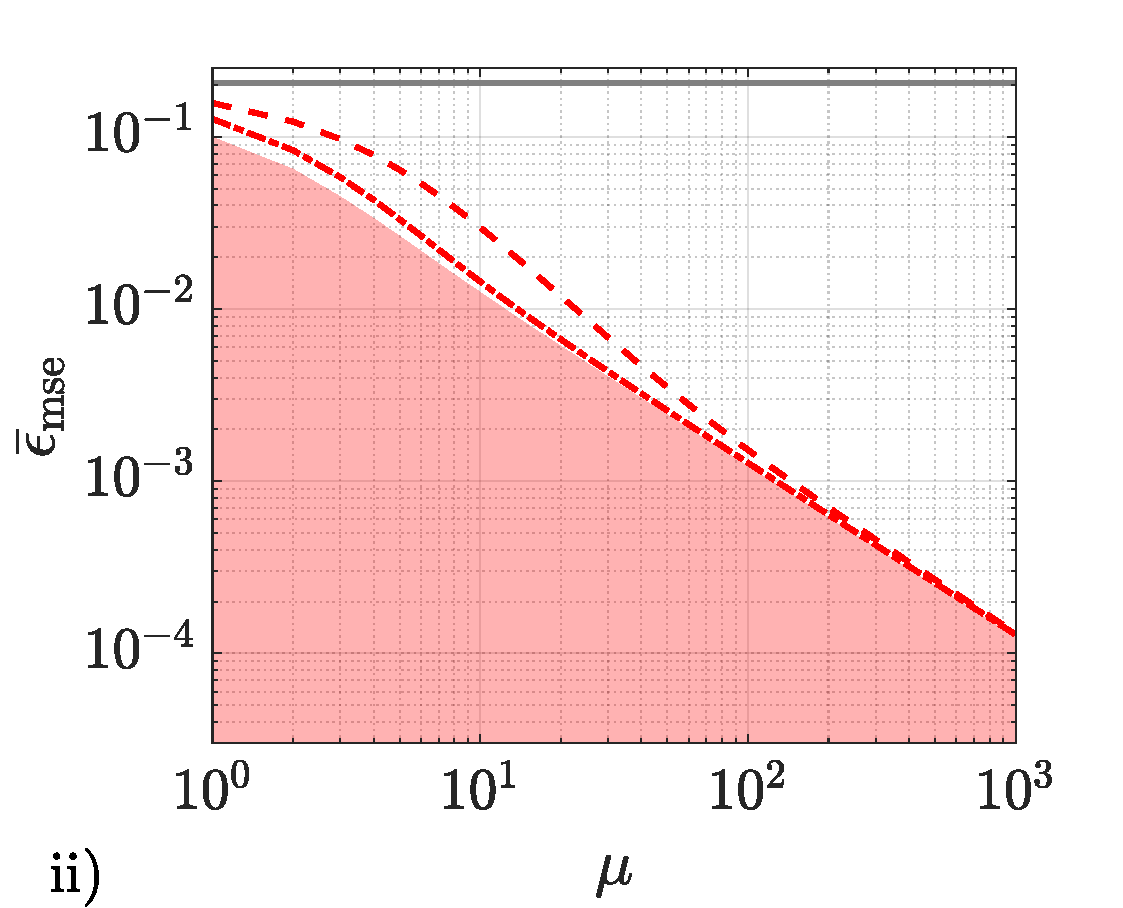
\includegraphics[trim={0.1cm 0.1cm 0.65cm 0.2cm},clip,width=7.7cm]{ch5_fig6ii}
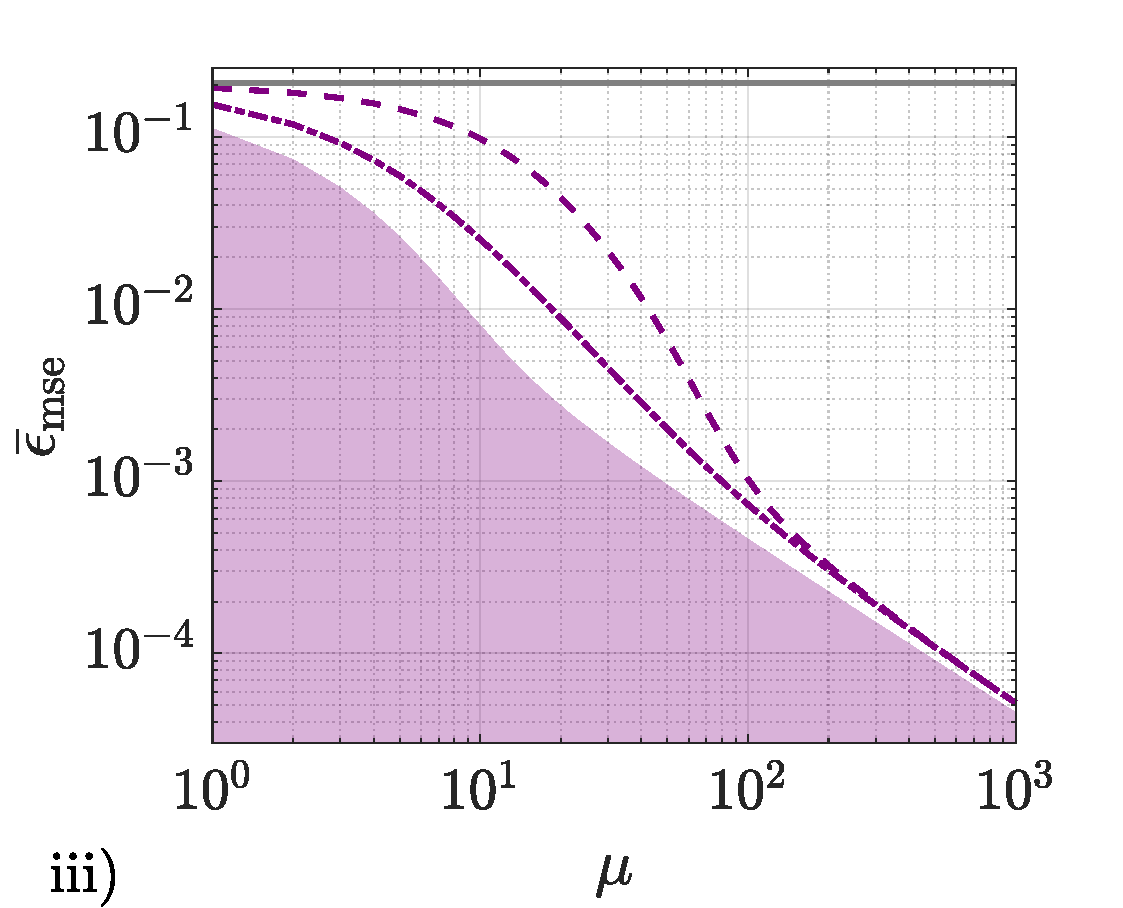
\includegraphics[trim={0.1cm 0.1cm 0.65cm 0.2cm},clip,width=7.7cm]{ch5_fig6iii}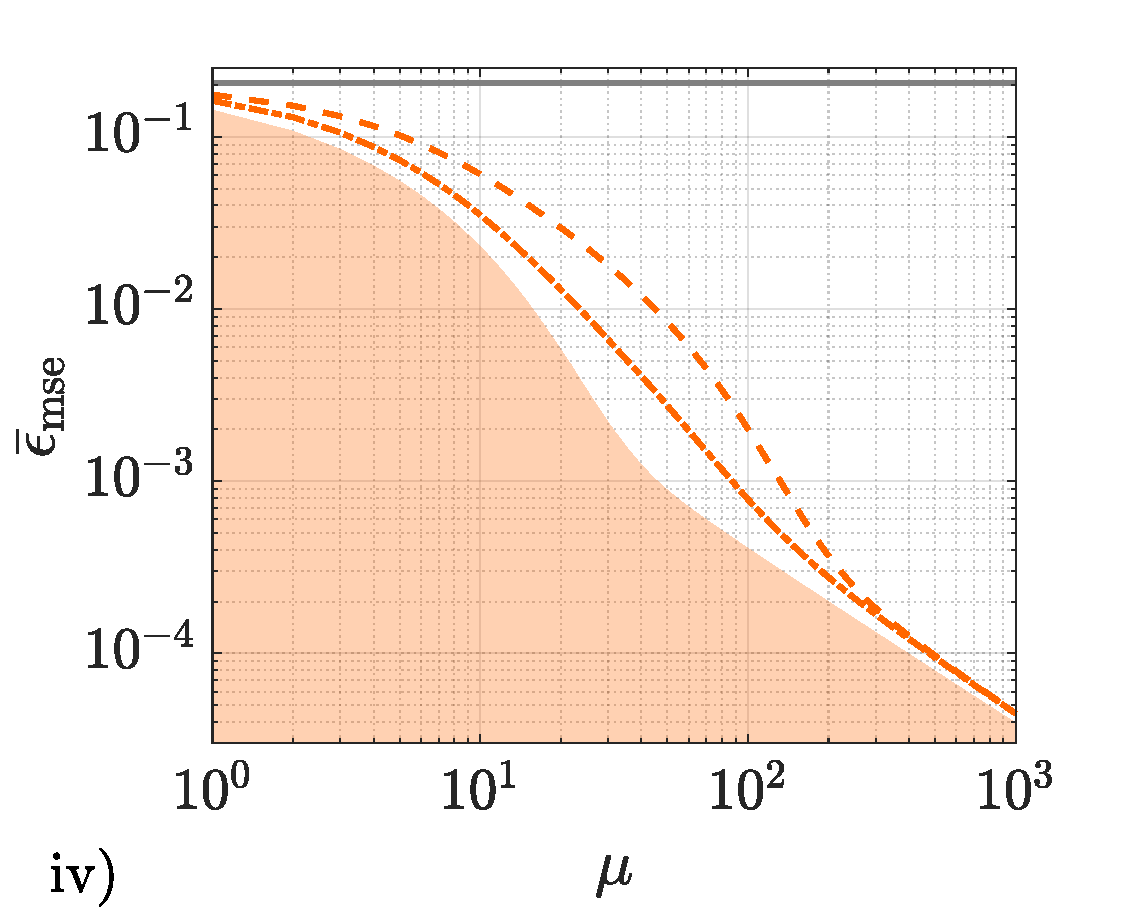
\includegraphics[trim={0.1cm 0.1cm 0.65cm 0.2cm},clip,width=7.7cm]{ch5_fig6iv}
	\caption[Performance of schemes with practical states and POMs]{i) Mean square error based on the optimal single-shot strategy (shaded area), error associated with the measurement of energy (dashed line) and prior variance (horizontal solid line) for the coherent state, (ii) the twin squeezed vacuum state, (iii) the squeezed entangled state, and (iv) the twin squeezed cat state, with mean number of photons $\bar{n}=2$, prior mean $\bar{\theta} = 0$ and prior width $W_0 = \pi/2$. Furthermore, the dash-dot graphs in (ii), (iii) and (iv) represents the uncertainty for the measurement of quadratures. The sequences of operations that implement the POMs that produce these results can be found in table \ref{POM_summary}.}
\label{continuousPOM}
\end{figure}

\begin{table} [t]
\centering
{\renewcommand{\arraystretch}{1.45} 
\begin{tabular}{|l|c|c|c|}
\hline
Measurement & Observable & Projectors  & States \\
\hline
\hline
\begin{tabular}{@{}l@{}}$50$:$50$ splitter \& \\ counting (even) \end{tabular} & \begin{tabular}{@{}c@{}} $N_1 N_2 = \int dk~k \ketbra{k}{k}$, \\ with $N_i = a_i^{\dagger}a_i$ \end{tabular} & $\left\lbrace\mathrm{e}^{-i\frac{\pi}{4}N_2}\mathrm{e}^{-i\frac{\pi}{2}J_x}\ket{k}\right\rbrace_{k}$ & \begin{tabular}{@{}c@{}} All but \\ coherent \end{tabular} \\
\hline
\begin{tabular}{@{}l@{}}$50$:$50$ splitter \& \\ counting (odd) \end{tabular} & \begin{tabular}{@{}c@{}}$N_1 N_2 = \int dk~ k \ketbra{k}{k}$, \\ with $N_i = a_i^{\dagger}a_i$ \end{tabular}& $\left\lbrace\mathrm{e}^{-i\frac{\pi}{2}N_2}\mathrm{e}^{-i\frac{\pi}{2}J_x}\ket{k}\right\rbrace_{k}$ & Coherent \\
\hline
$\pi/8$ quadratures & \begin{tabular}{@{}c@{}}$X_1 X_2 = \int dq~ q \ketbra{q}{q}$, with \\ $X_i = [ \mathrm{e}^{i \frac{\pi}{8}} a_i^{\dagger} + \mathrm{e}^{-i\frac{\pi}{8}}a_i]/\sqrt{2}$\end{tabular}  & $\left\lbrace\mathrm{e}^{i\frac{\pi}{4}N_1}\mathrm{e}^{-i\frac{\pi}{2}J_x}\ket{q}\right\rbrace_{q}$ &  \begin{tabular}{@{}c@{}} All but \\ coherent \end{tabular} \\
\hline 
\begin{tabular}{@{}l@{}}Undoing \& \\  counting\end{tabular} & $N_1 N_2 = \int dk~ k \ketbra{k}{k}$ & $\left\lbrace\mathrm{e}^{i \pi J_z }\mathrm{e}^{i\frac{\pi}{2}J_x}D_1^{\dagger}\left(\alpha\right)\ket{k}\right\rbrace_{k}$ & Coherent \\
\hline
Parity POMs & \begin{tabular}{@{}c@{}} $\Pi_1 \Pi_2 = \int dp~ p \ketbra{p}{p}$, \\ with $\Pi_i = (-1)^{a_i^{\dagger}a_i}$ \end{tabular}& $\left\lbrace\mathrm{e}^{-i\frac{\pi}{4}N_2}\mathrm{e}^{-i\frac{\pi}{2}J_x}\ket{p}\right\rbrace_{p}$ & NOON \\ 
\hline
\end{tabular}}
\caption[Practical POMs to approach our non-asymptotic quantum bounds]{Sequences of quantum operations needed to implement the practical measurements discussed in section \ref{measurements_section}, whose uncertainty is represented in figures \ref{continuousPOM} and \ref{noonPOM}. Note that the observable column indicates the physical quantity that is being measured, and that the different combinations of phase shifts that appear in the third column have been chosen such that the schemes are optimal when the prior is centred around $\bar{\theta} = 0$ and $\bar{n} = 2$.}
\label{POM_summary}
\end{table}

To start our discussion of the low trial number regime with this POM, we first observe that, according to figure \ref{continuousPOM}.i, measuring energy with coherent states produces an uncertainty that is already very close to the associated bound for a low value of $\mu$. More concretely, the bound and the measurement error only differ in their second and third significant figures, as can be directly verified from the values in table \ref{practical_POM_summary}, where we provide the numerical uncertainties for the first ten shots of every scheme based on indefinite photon number strategies. Moreover, this can be further improved if instead we undo the preparation of the probe state before counting photons, that is, by reversing the $50$:$50$ beam splitter and the displacement from the vacuum operations that generated the coherent state in the first place. The extra known difference of phases showed in table \ref{POM_summary} is also needed for the case with $\bar{\theta}=0$ that we are considering. Nonetheless, taking into account the fact that both schemes produce an uncertainty whose first significant figure is that of the optimum (see table \ref{practical_POM_summary}), we conclude that, for most practical purposes, they are equally useful and optimal given any number of repetitions. 

\begin{table} [t]
\centering
{\renewcommand{\arraystretch}{1.2} 
\begin{tabular}{|c|c|c|c|c|c|}
\hline
\multicolumn{6}{|c|}{$\bar{\epsilon}_{\mathrm{mse}}\left(\mu = 1\right)$, $\dots$, $\bar{\epsilon}_{\mathrm{mse}}\left(\mu = 10 \right)$} \\
\hline
\hline
\multicolumn{3}{|c|}{Coherent state} & \multicolumn{3}{c|}{Twin squeezed vacuum state} \\
\hline
\begin{tabular}{@{}c@{}}Single-shot \\ POM\end{tabular} & \begin{tabular}{@{}c@{}}$50$:$50$ splitter \\ \& counting\end{tabular} & \begin{tabular}{@{}c@{}}Undoing \& \\ counting\end{tabular} & \begin{tabular}{@{}c@{}}Single-shot \\ POM\end{tabular} & \begin{tabular}{@{}c@{}}$50$:$50$ splitter \\ \& counting\end{tabular} & \begin{tabular}{@{}c@{}} $\pi/8$ \\ quadra. \end{tabular} \\
\hline
$1.44\cdot 10^{-1}$ & $1.49\cdot 10^{-1}$ & $1.47\cdot 10^{-1}$ & $9.94\cdot 10^{-2}$ & $1.57\cdot 10^{-1}$ & $1.27\cdot 10^{-1}$ \\
$1.11\cdot 10^{-1}$ & $1.15\cdot 10^{-1}$ & $1.13\cdot 10^{-1}$ & $6.48\cdot 10^{-2}$ & $1.23\cdot 10^{-1}$ & $8.37\cdot 10^{-2}$ \\
$8.94\cdot 10^{-2}$ & $9.25\cdot 10^{-2}$ & $9.07\cdot 10^{-2}$ & $4.49\cdot 10^{-2}$ & $9.71\cdot 10^{-2}$ & $5.83\cdot 10^{-2}$ \\
$7.47\cdot 10^{-2}$ & $7.70\cdot 10^{-2}$ & $7.56\cdot 10^{-2}$ & $3.36\cdot 10^{-2}$ & $7.85\cdot 10^{-2}$ & $4.31\cdot 10^{-2}$ \\
$6.40\cdot 10^{-2}$ & $6.59\cdot 10^{-2}$ & $6.47\cdot 10^{-2}$ & $2.64\cdot 10^{-2}$ & $6.44\cdot 10^{-2}$ & $3.32\cdot 10^{-2}$ \\
$5.60\cdot 10^{-2}$ & $5.74\cdot 10^{-2}$ & $5.66\cdot 10^{-2}$ & $2.17\cdot 10^{-2}$ & $5.38\cdot 10^{-2}$ & $2.67\cdot 10^{-2}$ \\
$4.98\cdot 10^{-2}$ & $5.10\cdot 10^{-2}$ & $5.02\cdot 10^{-2}$ & $1.83\cdot 10^{-2}$ & $4.56\cdot 10^{-2}$ & $2.22\cdot 10^{-2}$ \\
$4.48\cdot 10^{-2}$ & $4.58\cdot 10^{-2}$ & $4.51\cdot 10^{-2}$ & $1.58\cdot 10^{-2}$ & $3.91\cdot 10^{-2}$ & $1.89\cdot 10^{-2}$ \\
$4.07\cdot 10^{-2}$ & $4.15\cdot 10^{-2}$ & $4.10\cdot 10^{-2}$ & $1.40\cdot 10^{-2}$ & $3.39\cdot 10^{-2}$ & $1.64\cdot 10^{-2}$ \\
$3.74\cdot 10^{-2}$ & $3.80\cdot 10^{-2}$ & $3.76\cdot 10^{-2}$ & $1.25\cdot 10^{-2}$ & $2.98\cdot 10^{-2}$ & $1.45\cdot 10^{-2}$ \\
\hline
\hline
\multicolumn{3}{|c|}{Squeezed entangled state} & \multicolumn{3}{c|}{Twin squeezed cat state} \\
\hline
\begin{tabular}{@{}c@{}}Single-shot \\ POM\end{tabular} & \begin{tabular}{@{}c@{}}$50$:$50$ splitter \\ \& counting\end{tabular} & \begin{tabular}{@{}c@{}} $\pi/8$ \\ quadra. \end{tabular} & \begin{tabular}{@{}c@{}}Single-shot \\ POM\end{tabular} & \begin{tabular}{@{}c@{}}$50$:$50$ splitter \\ \& counting\end{tabular} & \begin{tabular}{@{}c@{}} $\pi/8$ \\ quadra. \end{tabular} \\
\hline 
$1.12\cdot 10^{-1}$ & $1.93\cdot 10^{-1}$ & $1.54\cdot 10^{-1}$ & $1.43\cdot 10^{-1}$ & $1.76\cdot 10^{-1}$ & $1.62\cdot 10^{-1}$ \\
$7.38\cdot 10^{-2}$ & $1.80\cdot 10^{-1}$ & $1.18\cdot 10^{-1}$ & $1.08\cdot 10^{-1}$ & $1.52\cdot 10^{-1}$ & $1.30\cdot 10^{-1}$ \\
$5.08\cdot 10^{-2}$ & $1.68\cdot 10^{-1}$ & $9.23\cdot 10^{-2}$ & $8.46\cdot 10^{-2}$ & $1.32\cdot 10^{-1}$ & $1.06\cdot 10^{-1}$ \\
$3.60\cdot 10^{-2}$ & $1.56\cdot 10^{-1}$ & $7.34\cdot 10^{-2}$ & $6.77\cdot 10^{-2}$ & $1.16\cdot 10^{-1}$ & $8.75\cdot 10^{-2}$ \\
$2.62\cdot 10^{-2}$ & $1.45\cdot 10^{-1}$ & $5.95\cdot 10^{-2}$ & $5.53\cdot 10^{-2}$ & $1.02\cdot 10^{-1}$ & $7.33\cdot 10^{-2}$ \\
$1.96\cdot 10^{-2}$ & $1.34\cdot 10^{-1}$ & $4.87\cdot 10^{-2}$ & $4.56\cdot 10^{-2}$ & $9.08\cdot 10^{-2}$ & $6.22\cdot 10^{-2}$ \\
$1.51\cdot 10^{-2}$ & $1.24\cdot 10^{-1}$ & $4.06\cdot 10^{-2}$ & $3.81\cdot 10^{-2}$ & $8.13\cdot 10^{-2}$ & $5.33\cdot 10^{-2}$ \\
$1.19\cdot 10^{-2}$ & $1.15\cdot 10^{-1}$ & $3.43\cdot 10^{-2}$ & $3.19\cdot 10^{-2}$ & $7.33\cdot 10^{-2}$ & $4.60\cdot 10^{-2}$ \\
$9.65\cdot 10^{-3}$ & $1.06\cdot 10^{-1}$ & $2.94\cdot 10^{-2}$ & $2.70\cdot 10^{-2}$ & $6.65\cdot 10^{-2}$ & $4.01\cdot 10^{-2}$ \\
$8.04\cdot 10^{-3}$ & $9.77\cdot 10^{-2}$ & $2.54\cdot 10^{-2}$ & $2.30\cdot 10^{-2}$ & $6.07\cdot 10^{-2}$ & $3.52\cdot 10^{-2}$ \\
\hline
\end{tabular}}
\caption[Numerical results for the indefinite photon number states]{Mean square error for the indefinite photon number states using the optimal single-shot POM and the physical measurement schemes described in the main text, with $1\leqslant\mu\leqslant 10$, $\bar{n}=2$, $\bar{\theta}=0$ and $W_0=\pi/2$.}
\label{practical_POM_summary}
\end{table}

The situation is very different when we consider the other three states in figures \ref{continuousPOM}.ii - \ref{continuousPOM}.iv, where the uncertainty of the energy measurement is now notably higher than each bound in the regime of limited data, the distance between the graphs of the measurement and those of the bounds being larger for a few repetitions than for a single shot. This measurement is particularly detrimental for the strategy based on the squeezed entangled state, since its error is very close to the prior variance (horizontal line in \ref{continuousPOM}.iii) when $\mu \sim 1$ and this indicates that almost no information is being gained there. Additionally, we can observe that the twin squeezed cat state in figure \ref{continuousPOM}.ii presents a slow convergence to the asymptotic Cram\'{e}r-Rao bound when we use this POM, compared with the twin squeezed vacuum probe state in figure \ref{continuousPOM}.ii or the coherent state in in figure \ref{continuousPOM}.i. Note that this is the same problem found in section \ref{subsec:uncertaintynonasymptotic} for the squeezed entangled state, which is also reproduced in our calculations here.

These results show that counting photons is not the best strategy to be followed when $\mu$ is low and the probes have been prepared in states with a large Fisher information such as the ones considered here, and this motivates the search for other practical alternatives. More concretely, instead of projecting onto the energy basis, we can consider the measurement of a different physical quantity. The dash-dot lines in figures \ref{continuousPOM}.ii - \ref{continuousPOM}.iv show the results where we have projected onto the eigenstates of the observable $X_1\otimes X_2$,
\begin{equation}
X_i =\frac{1}{\sqrt{2}}\left(a_i^\dagger \mathrm{e}^{i\pi/8} + a_i \mathrm{e}^{-i\pi/8}\right)
\label{quadrature}
\end{equation}
being a quadrature rotated by $\pi/8$ for the $i$-th mode \cite{barnett2002}, after having introduced the phase shift $\mathrm{exp}(i \frac{\pi}{4}a_1^\dagger a_1)$ and having applied a $50$:$50$ beam splitter (see table \ref{POM_summary})\footnote{Note that the eigenstates of the quadrature operator in equation (\ref{quadrature}) cannot be normalised \cite{barnett2002}, and that the eigenvectors mentioned in the main text refer to the numerical approximation associated with the truncated state that we are employing here.}. The error of this scheme also depends on $\bar{\theta}$.

By comparing the energy and quadrature POMs figures \ref{continuousPOM}.ii - \ref{continuousPOM}.iv we see that the graphs based on the latter measurement are substantially closer to the bounds than those for the former POM when the experiment is operating in the regime of limited data. In other words, we have found a physical measurement that improves over the results based on measuring the energy for the practical states under consideration and a low number of trials. Interestingly, the dash-dot lines still converge to the fundamental asymptotic bound, and this implies that in the asymptotic regime both schemes are, nevertheless, equivalent in practice and optimal.   

Although these results extend our findings in chapter \ref{chap:nonasymptotic}, figures \ref{continuousPOM}.ii - \ref{continuousPOM}.iv also show that it could still be possible to find other physical schemes with a better precision when $\mu$ is low, with a faster rate of convergence to the asymptotic minimum or even saturating the bound for any $\mu$. These are some of the questions that should be addressed for further progress in the design of experimentally feasible protocols that operate both in and out of the regime of limited data. 

\subsection{Optimality of NOON states}
\label{subsec:optnoon}

The fact that NOON states are conceptually simple makes them an excellent tool to understand metrology protocols, which is why we have chosen to study them separately. They emerge as the optimal probe that maximises the Fisher information over the definite photon number states \cite{demkowicz2011, jarzyna2016thesis}, and while they are unsuitable for a global estimation due to the multi-peak structure associated with the posterior probabilities that they generate (\cite{jarzyna2016thesis, kolodynski2014} and our analysis in section \ref{subsec:prioranalysis}), and they require that the scaling of the prior variance is already $\sim 1/\bar{n}^2$ in order to achieve the same scaling that the Cram\'{e}r-Rao bound predicts \cite{berry2012infinite, hall2012}, the results in section \ref{subsec:uncertaintynonasymptotic} have shown that they can still be useful to a certain extent in the intermediate regime of prior knowledge and limited data when the number of photons is low and the POM is based on measuring the energy at each port. In addition, this moderate usefulness also holds for the repetition of the single-shot optimal strategy according to our results in figure \ref{bounds_results}.i, since the NOON state performs better than the twin squeezed cat state for $1\leqslant\mu\leqslant10$. By studying the performance of this probe for different physical measurements with respect to the non-asymptotic bound we will see that NOON states are also optimal in another sense. 

\FloatBarrier

\begin{figure}[t]
\centering
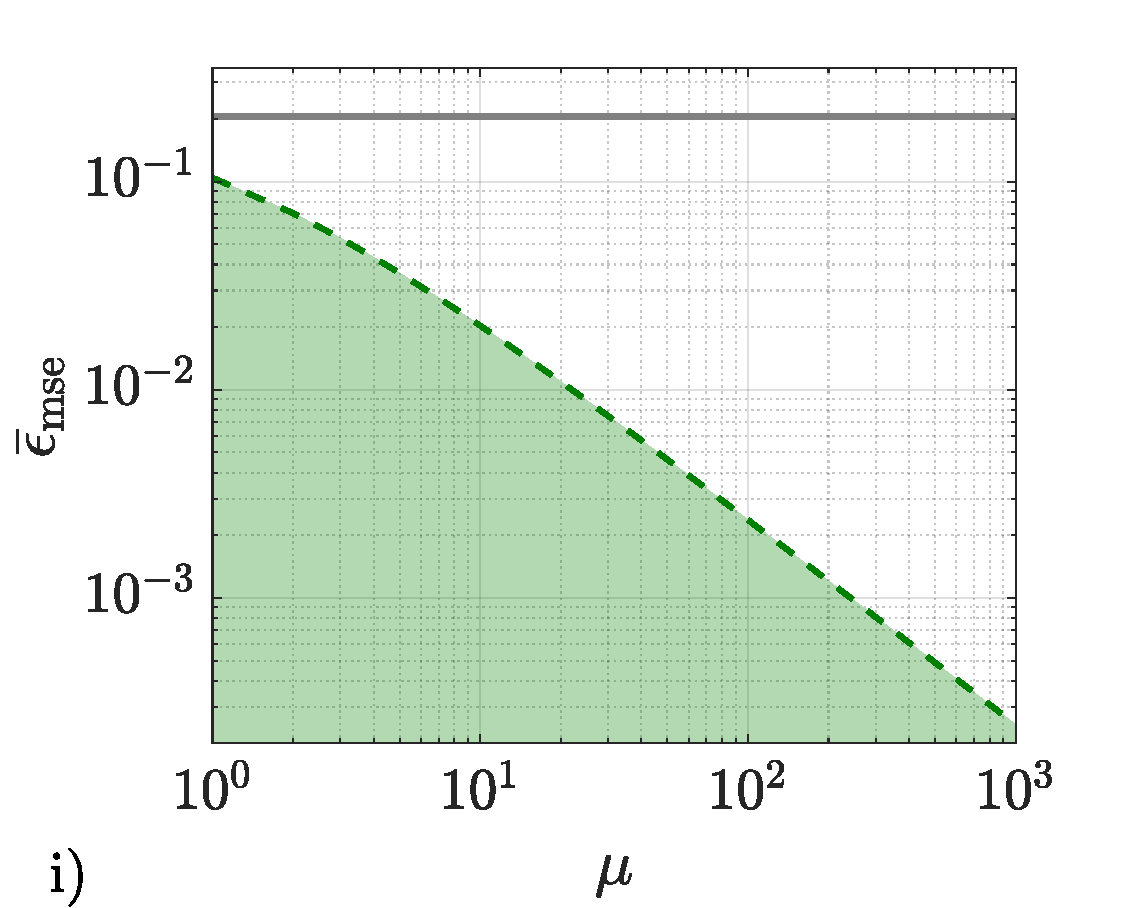
\includegraphics[trim={0.1cm 0.1cm 0.65cm 0.5cm},clip,width=7.7cm]{ch5_fig7i}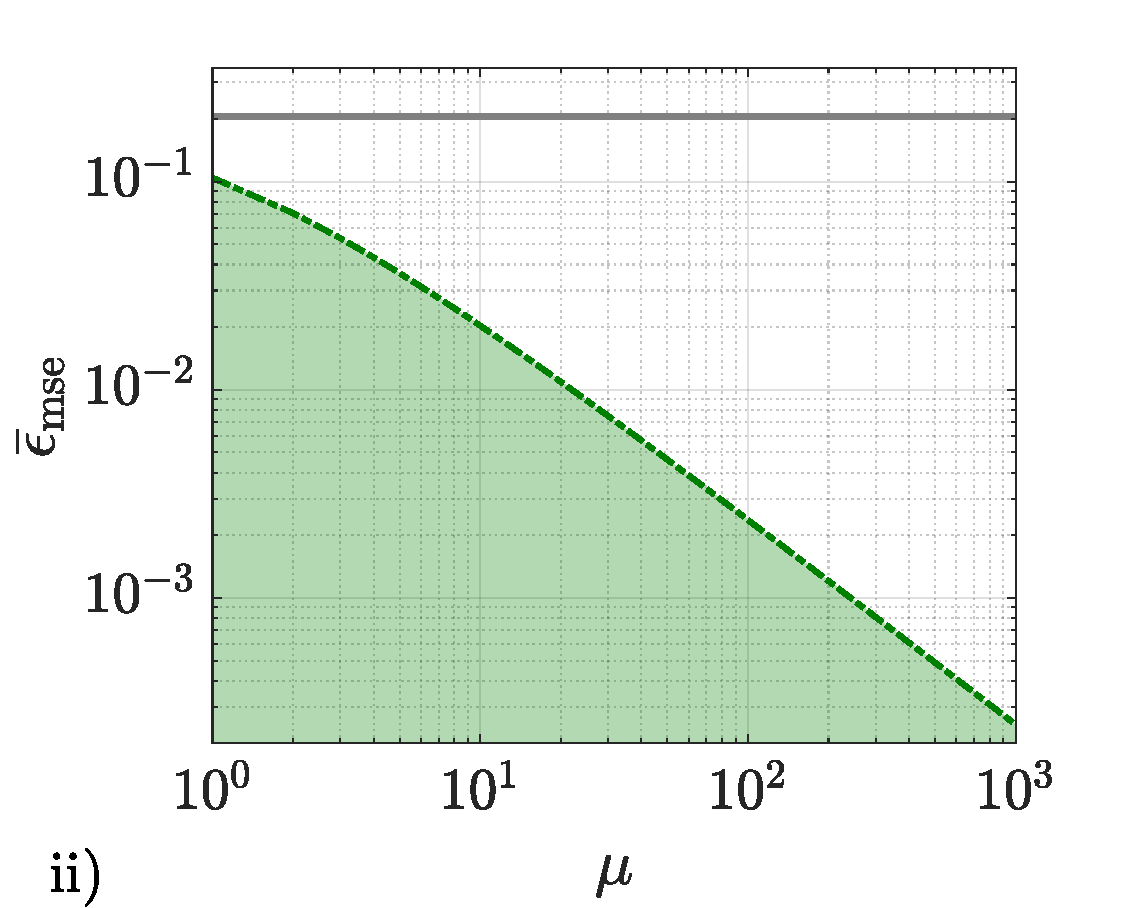
\includegraphics[trim={0.1cm 0.1cm 0.65cm 0.5cm},clip,width=7.7cm]{ch5_fig7ii}
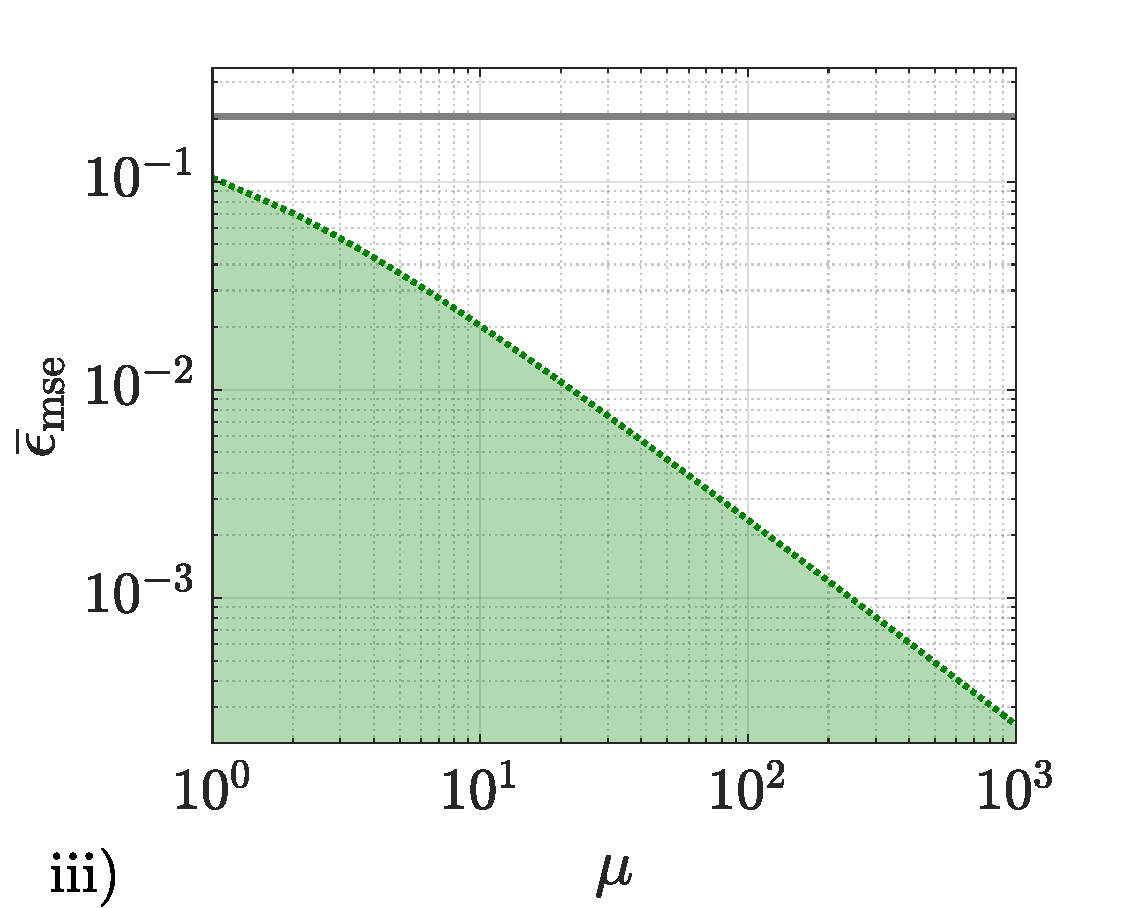
\includegraphics[trim={0.1cm 0.1cm 0.65cm 0.5cm},clip,width=7.7cm]{ch5_fig7iii}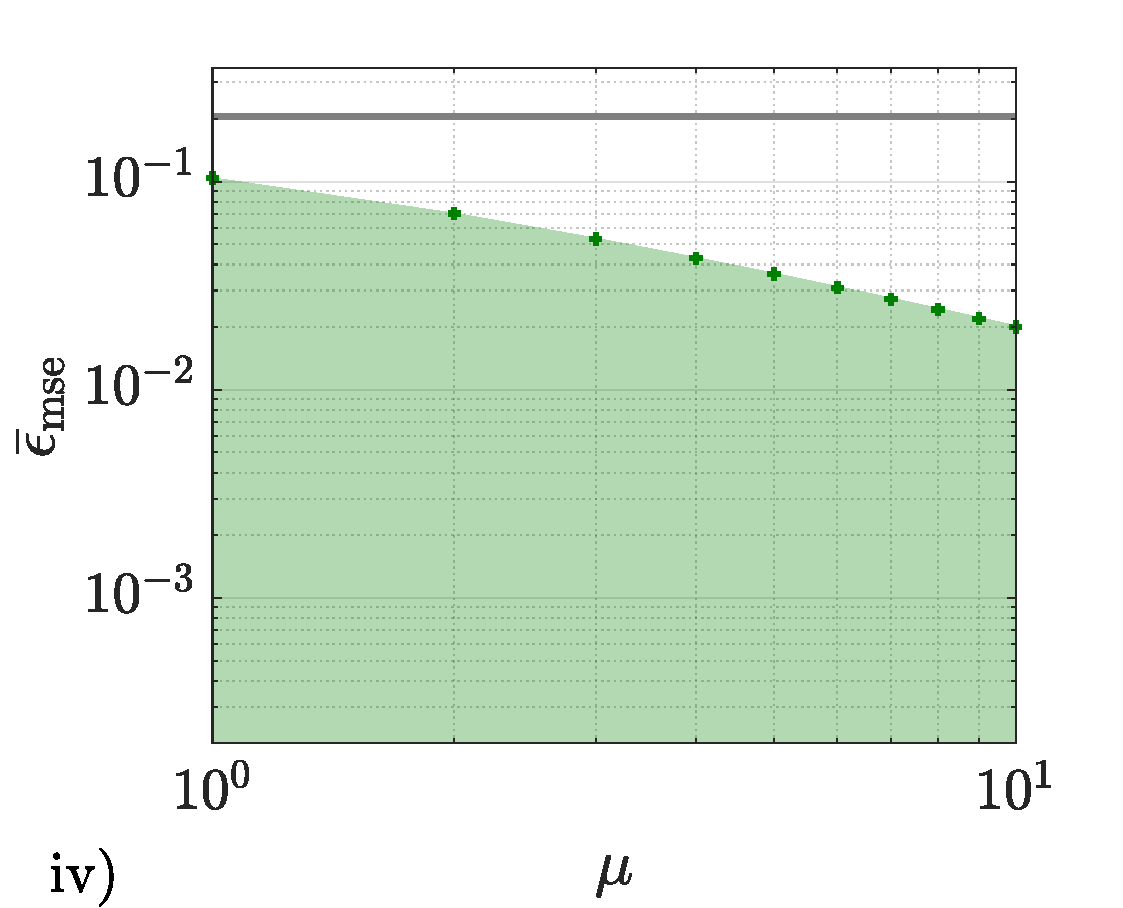
\includegraphics[trim={0.1cm 0.1cm 0.65cm 0.5cm},clip,width=7.7cm]{ch5_fig7iv}
	\caption[Performance of different POMs with a NOON probe state]{Mean square error based on the optimal single-shot strategy (shaded area), prior variance (horizontal solid line) and error associated with (i) the measurement of energy (dashed line), (ii) the measurement of quadratures (dash-dot line), (iii) parity measurements (dotted line), and (iv) the optimal collective measurement on $\mu$ copies of the probe (plus signs), for a NOON probe state with $\bar{n}=2$, $\bar{\theta} = 0$ and $W_0 = \pi/2$.}
\label{noonPOM}
\end{figure}

We start considering the two measurement schemes that we described in the previous section, that is, counting photons and measuring rotated quadratures after the introduction of some phase shifts that are indicated in table \ref{POM_summary}, and after the action of a $50$:$50$ beam splitter. The mean square errors generated by them for the NOON state, which are represented in figures \ref{noonPOM}.i and \ref{noonPOM}.ii, respectively, display a perfect agreement with the bounds for any number of repetitions. This can be further verified by observing that the numerical uncertainties for the first ten shots provided in table \ref{noon_POM_summary} are virtually identical. Additionally, for the photon counting measurement and a single shot it can be easily shown in an analytical fashion. To see it, first we calculate the likelihood function (see appendix \ref{sec:optrans}), finding that
\begin{eqnarray}
p(n,2-n|\theta) = \frac{\mathrm{cos}^2\left[\theta + (2n-3)\pi/4\right]}{ n! (2-n)!}.
\label{noonlikelihoodlimited}
\end{eqnarray}
Recalling that $n = 0, 1, 2$, equation (\ref{noonlikelihoodlimited}) can be expressed as
\begin{equation}
p(2,0|\theta) = p(0,2|\theta) = \frac{1}{2}~\mathrm{sin}^2\left(\theta - \frac{\pi}{4}\right), ~~ p(1,1|\theta) = \mathrm{cos}^2\left(\theta - \frac{\pi}{4}\right).
\label{likelihood_noon}
\end{equation}
Next we need to find the normalisation term of Bayes theorem, that is,
\begin{equation}
p(n,2-N) = \frac{2}{\pi} \int_{-\pi/4}^{\pi/4} d\theta p(n,2-n|\theta).
\label{normalisationbayes}
\end{equation}
Introducing equation (\ref{likelihood_noon}) in the formula for $p(n,2-n)$ we find that $p(2,0) = p(0,2) = 1/4$ and $p(1,1)=1/2$. At the same time, this gives us the last piece that we need to apply Bayes theorem and find the posterior probability $p(\theta|n,2-n) = p(\theta)p(n,2-n|\theta)/p(n,2-n)$, which in our case is
\begin{equation}
p(\theta|2,0) = p(\theta|0,2) = \frac{4}{\pi}\hspace{0.1em}\mathrm{sin}^2\left(\theta - \frac{\pi}{4}\right), ~~ p(\theta|1,1) = \frac{4}{\pi}\hspace{0.1em}\mathrm{cos}^2\left(\theta - \frac{\pi}{4}\right).
\label{posterior_noon}
\end{equation}
Now we observe that it is possible to rewrite the classically-optimal single-shot mean square error in equation (\ref{classicalbound}) as
\begin{equation}
\bar{\epsilon}_{\mathrm{mse}}(\mu=1) = \int d\theta p(\theta) \theta^2 - \int dn~ p(n,2-n) g_{\mathrm{opt}}(n,2-n)^2,
\end{equation}
where
\begin{equation}
g_{\mathrm{opt}}(n,2-n) = \int_{-\pi/4}^{\pi/4} d\theta p(\theta|n,2-n)\theta
\end{equation}
is the optimal estimator. Taking into account that $g_{\mathrm{opt}}(2,0) = g_{\mathrm{opt}}(0,2) = -1/\pi$ and $g_{\mathrm{opt}}(1,1) = 1/\pi$, the error associated to this POM is
\begin{equation}
\bar{\epsilon}_{\mathrm{mse}}(\mu=1) = \frac{2}{\pi}\int_{-\pi/4}^{\pi/4} d\theta \theta^2 - \frac{1}{\pi^2} = \frac{\pi^2}{48} - \frac{1}{\pi^2}.
\label{msesingleshotoptnoon}
\end{equation}
On the other hand, the single shot quantum bound is, in this case,
\begin{equation}
\bar{\epsilon}_{\mathrm{mse}}(\mu=1) \geqslant \frac{2}{\pi}\int_{-\pi/4}^{\pi/4} d\theta \theta^2 - \mathrm{Tr}(\bar{\rho}S) =
\frac{\pi^2}{48} - \frac{1}{\pi^2},
\label{mse_analytical_noon}
\end{equation}
which is the exact value found in equation (\ref{msesingleshotoptnoon}) (see the calculation of $\bar{\rho}$ and $S$ for the NOON state in section \ref{main_results}). Hence, the measurement under consideration saturates the single-shot bound, as we expected\footnote{We also notice the agreement of $\pi^2/48 - 1/\pi^2 \approx 0.104$ with the numerical results showed in table \ref{noon_POM_summary}.}.

\begin{table} [t]
\centering
{\renewcommand{\arraystretch}{1.2} 
\begin{tabular}{|c|c|c|c|c|}
\hline 
\multicolumn{5}{|c|}{$\bar{\epsilon}_{\mathrm{mse}}\left(\mu = 1\right)$, $\dots$, $\bar{\epsilon}_{\mathrm{mse}}\left(\mu = 10 \right)$} \\
\hline
\hline
\multicolumn{5}{|c|}{NOON state} \\
\hline
\begin{tabular}{@{}c@{}}Single-shot \\ POM \end{tabular} & \begin{tabular}{@{}c@{}}$50$:$50$ splitter \\ \& counting\end{tabular} & \begin{tabular}{@{}c@{}}$\pi/8$  \\ quadra. \end{tabular}  &  \begin{tabular}{@{}c@{}}Parity \\ POMs \end{tabular} & \begin{tabular}{@{}c@{}}Collective \\ POMs \end{tabular} \\
\hline 
$1.04\cdot 10^{-1}$ & $1.04\cdot 10^{-1}$ & $1.04\cdot 10^{-1}$ & $1.04\cdot 10^{-1}$ & $1.04\cdot 10^{-1}$ \\
$7.06\cdot 10^{-2}$ & $7.06\cdot 10^{-2}$ & $7.06\cdot 10^{-2}$ & $7.06\cdot 10^{-2}$ & $7.02\cdot 10^{-2}$ \\
$5.36\cdot 10^{-2}$ & $5.36\cdot 10^{-2}$ & $5.36\cdot 10^{-2}$ & $5.35\cdot 10^{-2}$ & $5.31\cdot 10^{-2}$ \\
$4.33\cdot 10^{-2}$ & $4.33\cdot 10^{-2}$ & $4.33\cdot 10^{-2}$ & $4.32\cdot 10^{-2}$ & $4.28\cdot 10^{-2}$ \\
$3.63\cdot 10^{-2}$ & $3.63\cdot 10^{-2}$ & $3.63\cdot 10^{-2}$ & $3.63\cdot 10^{-2}$ & $3.59\cdot 10^{-2}$ \\
$3.14\cdot 10^{-2}$ & $3.13\cdot 10^{-2}$ & $3.13\cdot 10^{-2}$ & $3.13\cdot 10^{-2}$ & $3.09\cdot 10^{-2}$ \\
$2.76\cdot 10^{-2}$ & $2.76\cdot 10^{-2}$ & $2.76\cdot 10^{-2}$ & $2.76\cdot 10^{-2}$ & $2.72\cdot 10^{-2}$ \\
$2.46\cdot 10^{-2}$ & $2.46\cdot 10^{-2}$ & $2.46\cdot 10^{-2}$ & $2.46\cdot 10^{-2}$ & $2.43\cdot 10^{-2}$ \\
$2.23\cdot 10^{-2}$ & $2.23\cdot 10^{-2}$ & $2.23\cdot 10^{-2}$ & $2.23\cdot 10^{-2}$ & $2.20\cdot 10^{-2}$ \\
$2.03\cdot 10^{-2}$ & $2.03\cdot 10^{-2}$ & $2.03\cdot 10^{-2}$ & $2.03\cdot 10^{-2}$ & $2.00\cdot 10^{-2}$ \\ 
\hline
\end{tabular}}
\caption[Numerical results for NOON states]{Mean square error for the NOON state using the optimal single-shot POM, the physical measurement schemes described in the main text and collective measurements, with $1\leqslant\mu\leqslant 10$, $\bar{n}=2$, $\bar{\theta}=0$ and $W_0=\pi/2$. We note that the calculation for collective measurements has been performed with a different numerical algorithm (see the Mathematica code in appendix \ref{sec:singleshotalgorithm}).}
\label{noon_POM_summary}
\end{table}

Similarly, a parity measurement based on the projectors of the observable $\Pi_1\otimes \Pi_2 =  (-1)^{a_1^{\dagger}a_1}\otimes (-1)^{a_2^{\dagger}a_2}$ \cite{gerry2010, chiruvelli2011}, and performed after introducing an extra phase shift and the action of a beam splitter (see table \ref{POM_summary}), also saturates the bound for all $\mu$, as it can be observed in figure \ref{noonPOM}.iii. This is consistent with the fact that the information about the phase is actually contained in the parity of the number of photons \cite{kolodynski2014, gerry2010, chiruvelli2011}. Interestingly, we have verified that counting photons and checking the parity at each port produces the same non-asymptotic results for the indefinite photon number states too. 

That different physical schemes are able to saturate the same quantum bound can be explained by recalling that the optimal quantum estimator $S$ is only defined on the support of $\rho$. In particular, for NOON states $\rho$ can be represented by a non-singular ($2 \times 2$) matrix in the number basis (see section \ref{main_results}), which is only a part of the full space including all the sectors with any number of photons. As a consequence, any measurement that coincides with the projectors $\ket{s_1}$ and $\ket{s_2}$ given in equation (\ref{noon_projectors}) in the part of the space that corresponds to the support of $\rho$ is going to be optimal, independently of the particular form of the POM elements. 

Furthermore, the same intuition can be used to understand why it is more difficult to saturate the bounds for indefinite photon number states in the non-asymptotic regime. For these states there is a non-zero probability of detecting any number of photons at each port of the interferometer, which implies that the optimal quantum estimator $S$ can be constrained in all the sectors of the operator space, and these constraints need to be fully satisfied to saturate the single-shot bound. However, as we accumulate more data we start to approach the quantum Cram\'{e}r-Rao bound, which is based on the equation $L(\theta) \rho(\theta) + \rho(\theta) L(\theta) = 2 \partial \rho(\theta)/\partial\theta$, and this equation only has a unique solution on the support of $\rho(\theta)$ \cite{genoni2008}, which in our case is simply a pure state. That is, finding physical measurements that saturate the asymptotic bounds is generally less demanding and, in fact, the errors of the physical measurements in figures \ref{continuousPOM}.i - \ref{continuousPOM}.iv converge to the fundamental bound. 

This state of affairs gives rise to an interesting situation. The Bayesian bounds in figure \ref{bounds_results}.i show that, in principle, the NOON state is not the best option among the probes that we are examining for any number of repetitions. In spite of this fact, if we compare the uncertainty associated with counting photons after undoing the preparation of a coherent state, the measurement of quadratures for the states based on the squeezing operator,  and any of the physical measurement previously discussed for the NOON state, then it can be shown that, in this case, the NOON state is the best probe when $1 \leqslant \mu \leqslant 3$. In particular, this conclusion can be extracted by inspection from tables \ref{practical_POM_summary} and \ref{noon_POM_summary}. This analysis highlights the importance of studying the possibility of saturating the theoretical bounds using realistic implementations in a particularly transparent way.

On the other hand, the mathematical simplicity of NOON states allows us to go one step further and study collective measurements \cite{jarzyna2015true, jarzyna2016thesis}. Until now this work has followed the model for repetitions that we introduced in section \ref{sec:problem}. However, we also saw that a more general possibility is to prepare $\mu$ identical copies of some probe and perform a single measurement on all of them at once. Given that repeating an experiment is generally easier than implementing collective techniques, it would interesting to find out whether collective POMs produce better uncertainties in those schemes whose associated calculations are tractable.

If we upgrade the optimal single-shot bound in equation (\ref{singleshot_bound}) to cover the collective case we find that
\begin{equation}
\bar{\epsilon}_\mathrm{mse} \geqslant \int d\theta p(\theta) \theta^2 - \mathrm{Tr}\left(\bar{\rho}_\mu S_\mu\right),
\label{singleshot_collective}
\end{equation} 
where now $S_\mu$ is given by $S_\mu \rho_\mu + \rho_\mu S_\mu = 2 \bar{\rho}_\mu$ with 
\begin{equation}
\rho_\mu = \int d\theta p(\theta) \smash[b]{ \underbrace{\rho(\theta) \otimes \cdots \otimes \rho(\theta)\,}_\text{$\mu$ times}}
\label{zerothmoment_collective}
\end{equation}
and
\begin{equation}
\bar{\rho}_\mu = \int d\theta p(\theta) \smash[b]{ \underbrace{\rho(\theta) \otimes \cdots \otimes \rho(\theta)\,}_\text{$\mu$ times}}\theta.
\label{firstmoment_collective}
\end{equation}
~\\[-10pt]

An algorithm to calculate equation (\ref{singleshot_collective}) for NOON states is proposed in appendix \ref{sec:singleshotalgorithm}, and its application for $1\leqslant \mu \leqslant 10$ results in the graph of figure \ref{noonPOM}.iv, which coincides with the bound generated by repeating the optimal strategy for a single probe\footnote{Unfortunately, it becomes numerically challenging to increase the number of copies, which is why we only consider $1\leqslant \mu \leqslant 10$ for this calculation.}. Numerically, this agreement occurs at least for the first significant figure, as it can be verified in table \ref{noon_POM_summary}. Thus we conclude that collective measurements do not provide a better performance than the practical measurements previously studied when we are working in the low-$\mu$ regime, each probe is prepared in a NOON state with $\bar{n} = 2$ and the prior width is $W_0=\pi/2$.

In summary, we have shown that there are measurements that can saturate the bound for the NOON state for all $\mu$ simultaneously. Consequently, NOON states do not only have a special status in the local regime, but also in the regime of limited data and moderate prior knowledge\footnote{In \cite{jarzyna2016thesis} it is argued that NOON states emerge as the optimal probe with a definite number of photons in the limit where the prior information dominates, something that is shown in \cite{demkowicz2011}, and it is concluded that, for that reason, using NOON states is almost useless in a practical Bayesian context. Although it is true that NOON states are limited due to the ambiguity that they introduce in the estimation and, more importantly, because of the difficulties to use them in real experiments \cite{schafermeier2018}, we draw attention to the fact that the regime where the prior knowledge may play a substantial role is relevant and useful whenever we need to make inferences from a practical scenario where only a low number of experiments can be performed.}. This can be explained by noticing that the optimal projectors for a single shot in equation (\ref{noon_projectors}) are the same that the projectors predicted by the symmetric logarithmic derivative that defines the quantum Fisher information \cite{kolodynski2014}. While this probe state is fragile and difficult to prepare in more realistic scenarios \cite{schafermeier2018}, these results are still interesting from a fundamental perspective, and they have helped us to understand the problems associated with saturating the bounds of more practical states that we need to overcome in the future. 

\section{Comparing our method with the alternative quantum bounds}
\label{sec:alternativevssingleshot}

The shot-by-shot strategy that we have constructed generates valid lower bounds for repetitive experiments. The fact that they are based on the single-shot optimum implies that, in a sense, they are fundamental in scenarios where the experiment is repeated, and we have seen that there is a constructive way of finding the theoretical POM that reaches them. 

A crucial aspect of our tool is that the calculations associated with it can be performed in an efficient way for practical schemes, having provided an algorithm with analytical and numerical components to achieve that goal. However, one could argue that some of the quantum bounds for low $\mu$ that we reviewed in section (\ref{subsec:alternativebounds}) are still computationally simpler, even when in general they also require a numerical treatment. In this section we analyse the relative merit of employing our strategy when the results generated by the latter are compared with the predictions of two alternative tools: the quantum Ziv-Zakai and Weiss-Weinstein bounds \cite{tsang2012, tsang2016}.

The Ziv-Zakai bound in equation (\ref{qzzb}) is already in a form that we can apply to our optical configuration, and the numerical algorithm that implements this operation can be found in appendix \ref{subsec:qzzbnum}. On the other hand, the Weiss-Weinstein bound in equation (\ref{qwwbpriorterm}) is expressed in terms of the quantity $f_c(s,\theta) = \int d\theta' p(\theta' + \theta)^s p(\theta')^{1-s}$, for $\lbrace \theta', p(\theta')\neq 0\rbrace$. A choice for $s$ that tends to produce tighter bounds is $s=1/2$ \cite{tsang2016, weinstein1988}, and we will also use it here. In that case, the previous quantity is simplified as $f_c(1/2,\theta) = \int d\theta' \sqrt{p(\theta' + \theta) p(\theta')}$, for $\lbrace \theta', p(\theta')\neq 0\rbrace$, which measures the overlap between the prior probability and a displaced version of it. For the flat prior of width $W_0$ that we are employing this overlap is simply $f_c(1/2,\theta) = 1-\abs{\theta}/W_0$. Consequently, the Weiss-Weinstein bound in equation (\ref{qwwbpriorterm}) becomes
\begin{equation}
\bar{\epsilon}_{\mathrm{mse}} \geqslant \sup_{\theta} \frac{\theta^2 \left(1-\frac{\theta}{W_0}\right)^2 \abs{f(\theta)}^{4\mu}/2}{\abs{f(\theta)}^{2\mu} - \left(1-\frac{2\theta}{W_0}\right)\mathrm{Re}\left\lbrace \left[f(\theta)^{2} {f(2\theta)}^{*}\right ]^\mu \right\rbrace},
\label{qwwbsimpler}
\end{equation}
with $0 \leqslant \theta < W_0 $. The algorithm to find this bound is provided in appendix \ref{subsec:qwwbnum}. 

\begin{figure}[t]
\centering
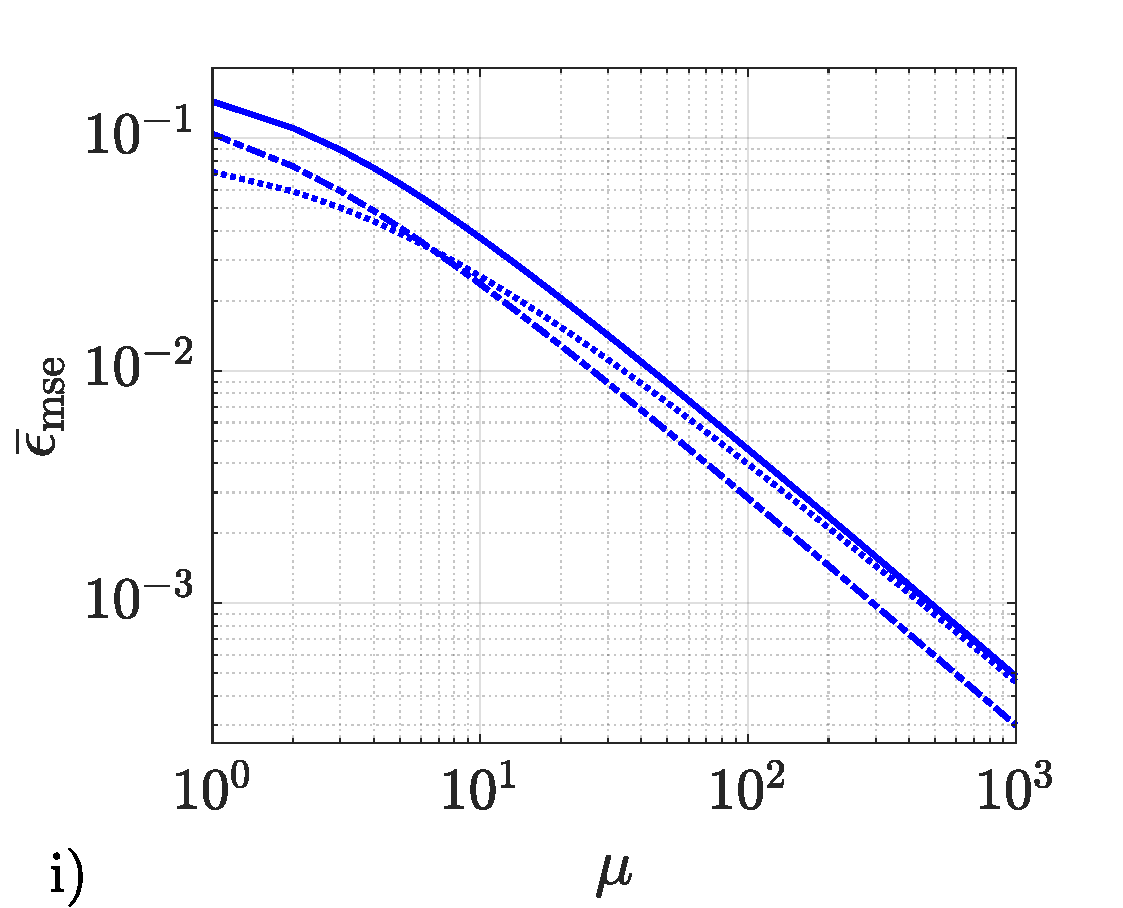
\includegraphics[trim={0.1cm 0.1cm 0.65cm 0.5cm},clip,width=7.7cm]{pictures/ch5_fig8i}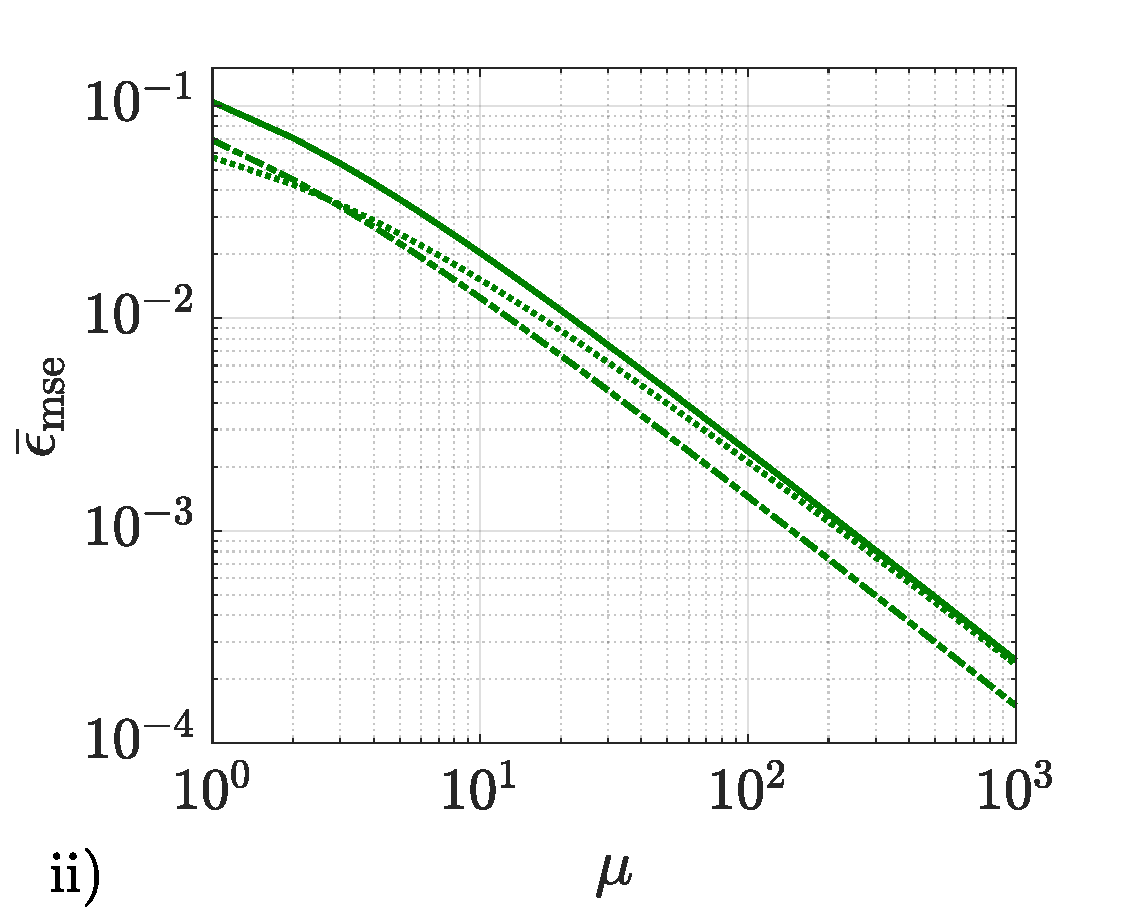
\includegraphics[trim={0.1cm 0.1cm 0.65cm 0.5cm},clip,width=7.7cm]{pictures/ch5_fig8ii}
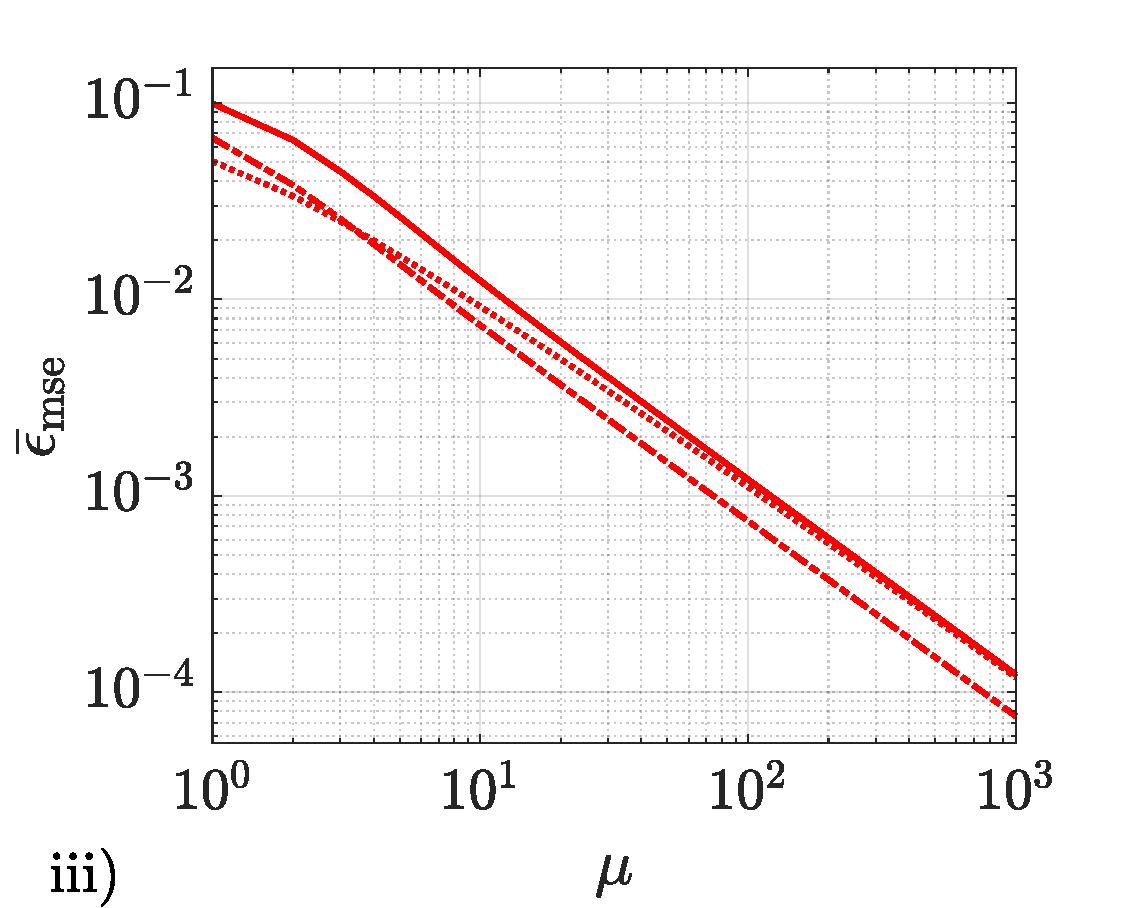
\includegraphics[trim={0.1cm 0.1cm 0.65cm 0.5cm},clip,width=7.7cm]{pictures/ch5_fig8iii}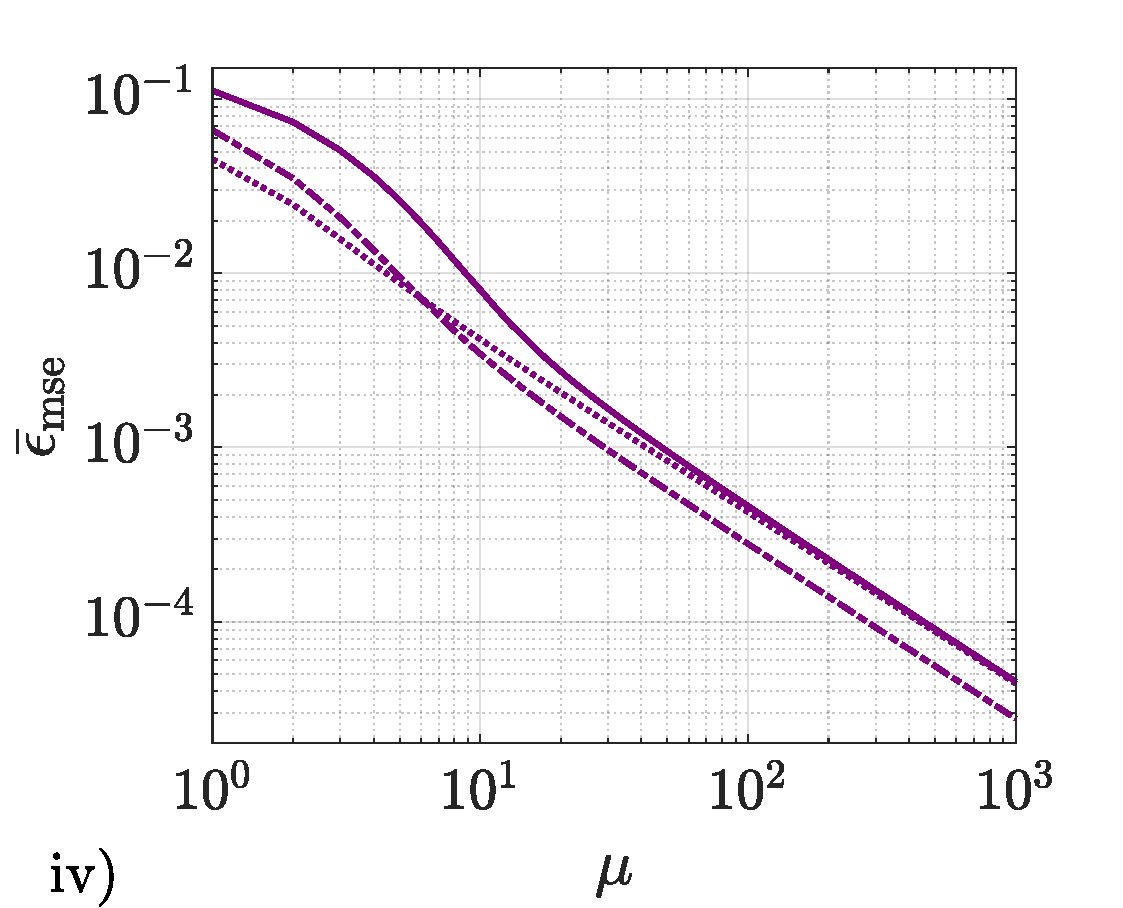
\includegraphics[trim={0.1cm 0.1cm 0.65cm 0.5cm},clip,width=7.7cm]{pictures/ch5_fig8iv}
\caption[Shot-by-shot bound versus Ziv-Zakai and Weiss-Weinstein]{Shot-by-shot strategy (solid line), quantum Ziv-Zakai bound (dash-dotted line) and quantum Weiss-Weinstein bound (dotted line) for (i) the coherent state, (ii) the NOON state, (iii) the twin squeezed vacuum state, and (iv) the squeezed entangled state, with $\bar{n} = 2$ and $W_{\mathrm{int}} = \pi/2$.}
\label{consistency}
\end{figure}

Figure \ref{consistency} shows the results of performing the previous calculations for (i) the coherent state, (ii) the NOON state, (iii) the twin squeezed entangled state and (iv) the twin squeezed cat state, where we have also included the bounds generated by repeating the single-shot optimal strategy (solid lines). As we can observe, neither the Ziv-Zakai bound (dash-dotted lines) nor the Weiss-Weinstein bound (dotted lines) coincides with with the single-shot optimum at $\mu = 1$, which means that these bounds are not tight in the single-shot regime. The Weiss-Weinstein bound is actually tight when $\mu \gg 1$, as it was proven in \cite{tsang2016}, while the Ziv-Zakai bound presents the correct scaling in this regime but it is not tight. Despite this, the latter bound is the tighter option when $\mu \sim 1$. 

The comparison for a low $\mu$ such that $\mu > 1$ is more subtle, since the bounds in equations (\ref{qzzb}) and (\ref{qwwbsimpler}) are defined for $\mu$ copies of the probe state, which in principle allows for collective measurements, while our bounds in section (\ref{sec:methodlimited}) are specifically designed for repetitions. Fortunately, we have been able to study collective techniques for NOON states, finding that both collective and repetitive measurements have the same precision for this configuration when $\mu$ is low. For that reason, the results for the NOON state in figure \ref{consistency}.ii demonstrate that the alternative bounds are loose in the intermediate regime. This implies that, in general, the quantum Ziv-Zakai and Weiss-Weinstein bounds are not tight in the non-asymptotic regime of optical metrology, in consistency with the examples in \cite{tsang2016}, and thus we conclude that our technique is preferred whenever we study repetitive experiments\footnote{Nonetheless, we observe that the quantum Ziv-Zakai and Weiss-Weinstein bounds correctly lower-bound the uncertainty for low values of $\mu$, in contrast to the Cram\'{e}r-Rao bound, since these bounds are valid for both biased and unbiased estimators \cite{tsang2012, tsang2016,  bayesbounds2007}.}. 

\section{Practical application: designing quantum experiments with genetic algorithms}
\label{sec:genetic}

The results in the previous sections, together with those in chapter \ref{chap:nonasymptotic}, complete our non-asymptotic methodology for single-parameter estimation problems. Now we would like to go a step further and conclude this chapter by exploiting our methods to design quantum states. In particular, we seek states that not only provide precision enhancements in the regime of limited data, but whose preparation is also associated with a concrete sequence of operations that can be implemented with current technology. Therefore, the findings in this section complement those in sections \ref{measurements_section} and \ref{subsec:optnoon}, where the sequences were only provided for POMs.

This problem belongs to the broader field of quantum state engineering, where ideas from machine learning and artificial intelligence are often utilised \cite{knott2016, jesus2018dec, driscoll2019}. In this context, Knott and his collaborators at Nottingham and Bristol \cite{jesus2018dec} proposed a genetic algorithm to design states in optical experiments. In what follows we show how the combination of these techniques with our methodology for single-parameter schemes provides a solution to the problem in the previous paragraph.

Let us first summarise the key ideas of the algorithm developed by Knott \emph{et al.} \cite{jesus2018dec}, which is called \emph{AdaQuantum}. One starts by creating a numerical toolbox with states, operations and measurements that can be performed with an optical arrangement. For example, the work \cite{jesus2018dec} includes a general splitter 
\begin{equation}
U_{ij}=\mathrm{exp}\left[\phi \left( a_i a_j^\dagger + a_i^\dagger a_j \right)\right]
\end{equation}
with transmissivity $T = \mathrm{cos}^2(\phi)$, the two-mode squeezing operator
\begin{equation}
S_{ij}=\mathrm{exp}\left(\zeta^{*}a_i a_j - \zeta a_i^\dagger a_j^\dagger\right)
\end{equation}
and the single-mode photon counting measurement $\ketbra{n}$, among others. 

The next step is to construct combinations of states, operations and measurements that together generate single-mode states. This is achieved by working in the space of $M$ modes and performing heralding measurements on $(M-1)$ of them, such that the state of the remaining mode is selected on the basis of the measurement outcome \cite{knott2016}. The results in this section have been obtained with $M = 2$. Then the final goal is to find arrangements of these experimental elements that give output states that are good for certain tasks, which is a search problem \cite{jesus2018dec}. 

Each of these combinations is said to be a \emph{genome}, and a collection of genomes is the \emph{population}. In addition, a \emph{fitness function} encoding the properties that we wish the final state to have is defined. This allows the algorithm to examine the values of such function for each of the genomes in the population, and to select those that are the fittest according to the criterion of the fitness function. The latter are then combined or modified, producing a new \emph{generation}, and the process is repeated until the probability of producing new improvements is very small.  

AdaQuantum, which was made available by its authors on GitHub \cite{adaquantum2019}, is flexible enough to accommodate different fitness functions, and this is precisely where our contribution starts. In particular, we prepared a MATLAB module including the numerical algorithms in appendices \ref{sec:singleshotalgorithm}, \ref{sec:pomnum} and \ref{sec:msematlab}, such that the Bayesian mean square error employed here could play the role of a fitness function in the regime of limited data and a realistic amount of prior knowledge. 

\begin{table} [t]
\centering
{\renewcommand{\arraystretch}{1.5} 
\begin{tabular}{|l|c|c|c|c|c|}
\hline
Setting & $\ket{\psi_{in}}$ & $\mathcal{O}_1$ & $\mathcal{O}_2$ & $\mathcal{O}_3$ & $\ketbra{n}$ \\
\hline
Ada, $\mu = 8$ & $|0,0\rangle$ & $S_{12}(\zeta = 0.89~\mathrm{e}^{i 0.031})$ & $U_{12}(T=0.69)$ &  $\mathrm{e}^{i N_1 0.32}$ & $\ketbra{4}$  \\
Ada, $\mu = 4$, $12$ & $|0,0\rangle$ & $S_{12}(\zeta = 0.91~\mathrm{e}^{i 0.040})$ & $U_{12}(T=0.66)$ & --- & $\ketbra{6}$ \\
Ada, $\mu = 1$ & $|0,0\rangle$ & $S_{12}(\zeta = 0.95~\mathrm{e}^{i 6.1})$ & $U_{12}(T=0.72)$ & --- & $\ketbra{2}$\\
\hline
\end{tabular}}
\caption[Sequences of quantum operations generated by AdaQuantum]{Details of the sequences generated by AdaQuantum using the Bayesian framework. The first two schemes are for a photon counting measurement after a $50$:$50$ beam splitter, and the last one is for the optimal single-shot POM. Note that $\ketbra{n}$ implements the heralding measurement that produces the single-mode state.}
\label{toolbox_summary}
\end{table}

Since AdaQuantum produces single-mode states and these cannot be used on its own because in experiments we can only access the information about the difference of phase shifts, one approach is to take a pair of such states as the input of our interferometer, that is, $\ket{\psi_0} = \ket{\psi}\otimes \ket{\psi}$, where $\ket{\psi}$ is the outcome of the genetic algorithm. The task given to AdaQuantum is thus to find the state $\ket{\psi}$ that minimises $\bar{\epsilon}_{\mathrm{mse}}$ for a given number of repetitions and measurement scheme. 

While the algorithm for the Bayesian error in appendix \ref{sec:msematlab} is relatively efficient when we only require the performance of a few schemes (section \ref{subsec:numalgorithm}), the genetic algorithm needs to calculate this error a large number of times in order to successfully evolve the optimal strategy through different generations, and this is numerically demanding. For that reason, we have chosen a narrow flat prior with $W_0 = \pi/12$ and $\bar{\theta} = 0$, so that the calculations associated with the integrals in equations (\ref{erropt}) and (\ref{shotbyshotmse}) for the mean square error are simplified\footnote{Notice that, according to our discussion in sections \ref{subsec:shotbyshot} and \ref{prior_section}, $W_0 = \pi/12 \approx 0.3$ is still a moderate amount of prior information.}. In addition, AdaQuantum assumes that $\bar{n} = 1$ for our configuration. As a consequence, the strategies in this section cannot be directly compared with those in the first part of this chapter.

We will optimise the error using two different strategies. First we focus on one of the practically-motivated POMs that we have studied: counting photons after the action of a $50$:$50$ beam splitter, including an extra phase shift that is known and that takes into account the fact that the prior is centred around zero\footnote{In particular, we have chosen its even version in table \ref{POM_summary}.}, and we set the algorithm to optimise the error for $\mu = 4$, $\mu = 8$ and $\mu = 12$ repetitions. This search produces a state that takes the form $\ket{\psi} = \mathcal{N}\langle n|\hat{U}_{12}\hat{S}_{12}|0,0\rangle$ for $\mu = 4$ and $\mu=12$, where $\mathcal{N}$ is the normalisation, while for $\mu = 8$ we find $\ket{\psi} = \mathcal{N}\langle n|\hat{P}_1\hat{U}_{12}\hat{S}_{12}|0,0\rangle$, where $P_1$ is a phase shift in the first mode. Table \ref{toolbox_summary} provides the numerical parameters for the sequences of operations that would prepare these states in practice, and the uncertainty associated with two copies of the previous probes has been represented in figure \ref{bmse_ada_results}.i (individual points). Furthermore, we have included the errors for the coherent state (solid line, CS) and the twin squeezed vacuum state (dashed line, SV), as references. The motivation to use the latter as a benchmark is that while it illustrates the potential enhancement that quantum resources can provide, it is also a common and well-understood probe state, in contrast with more exotic choices such as those studied in section \ref{sec:methodlimited}. 

\begin{figure}[t]
\centering
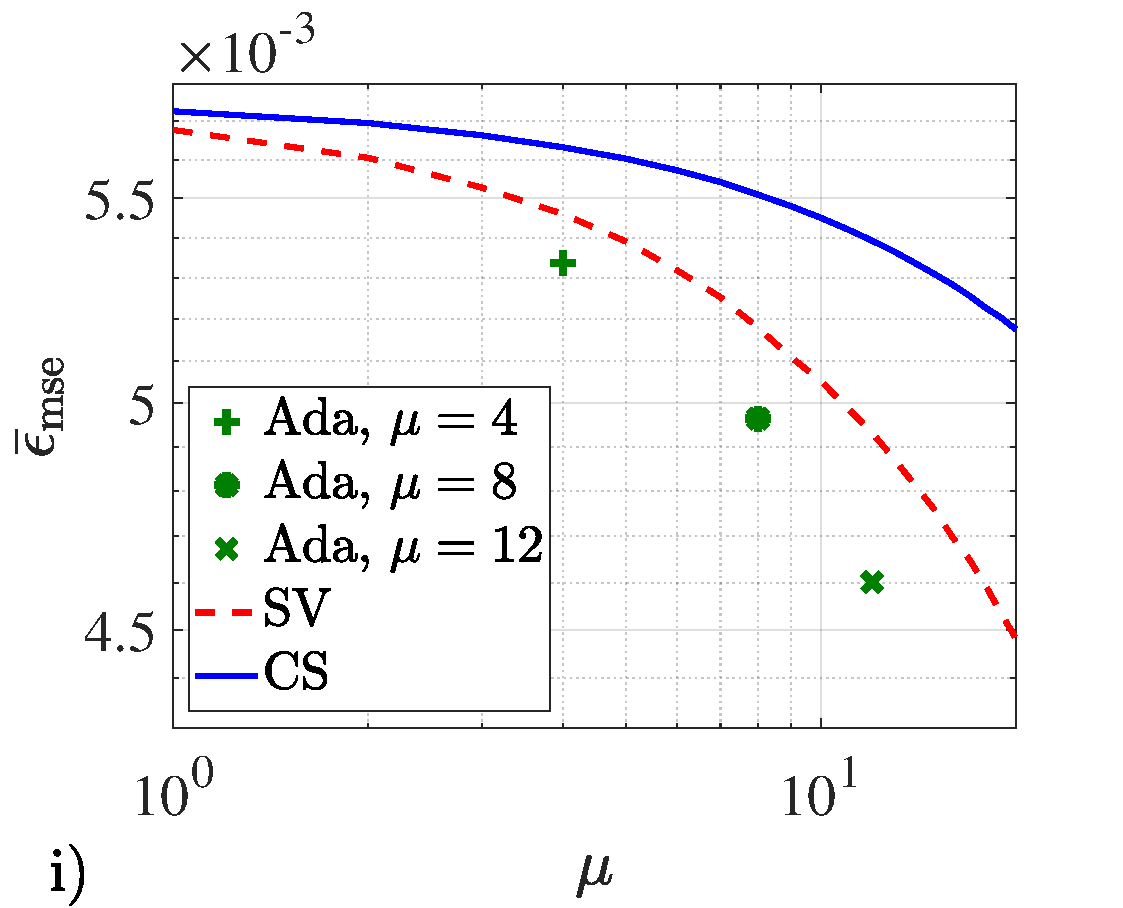
\includegraphics[trim={0.1cm 0.1cm 0.65cm 0.2cm},clip,width=7.7cm]{ch5_fig9i}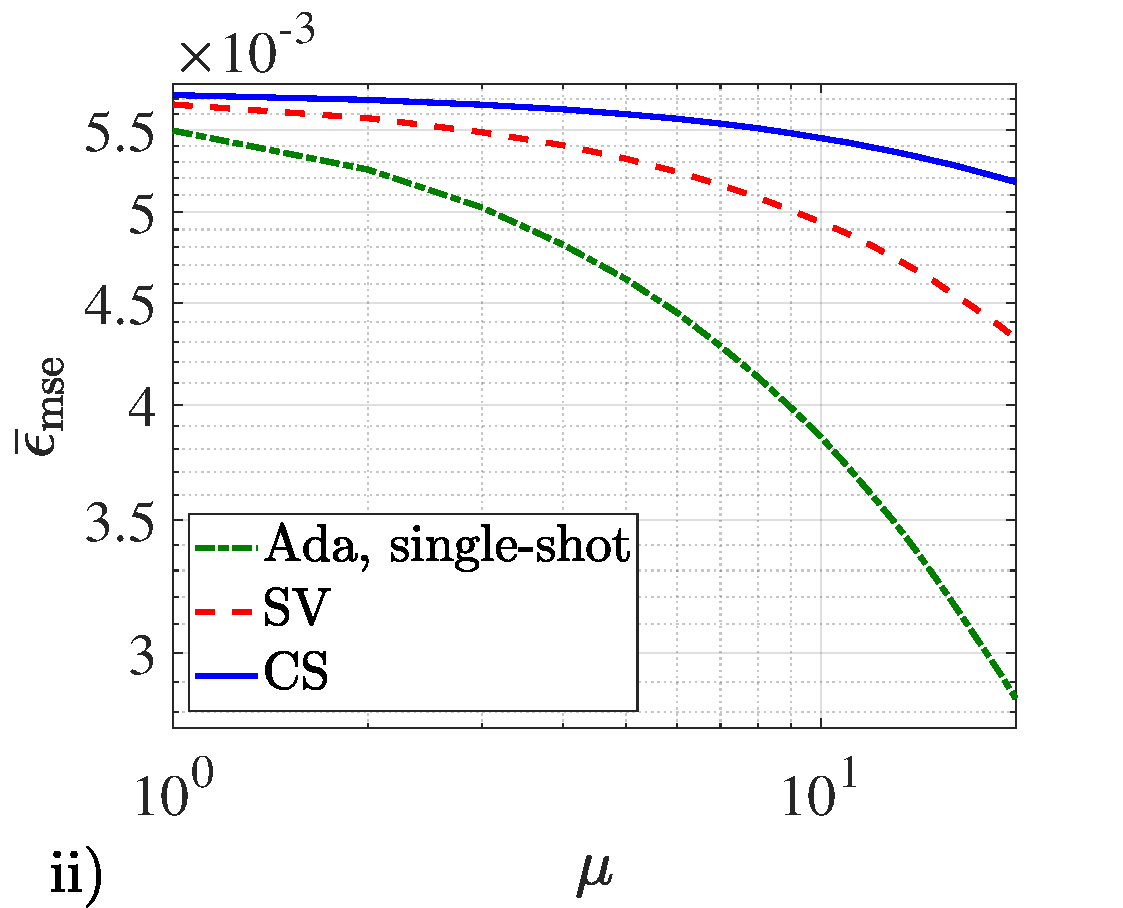
\includegraphics[trim={0.1cm 0.1cm 0.65cm 0.2cm},clip,width=7.7cm]{ch5_fig9ii}
\caption[Performance of the schemes found by AdaQuantum]{Mean square error as a function of the number of repetitions for (i) the coherent state (solid line, CS), the twin squeezed vacuum (dashed line, SV) and the states found by AdaQuantum for $\mu = 4$ (plus sign), $\mu = 8$ (asterisk) and $\mu = 12$ (cross) repetitions. Here the measurement scheme is based on counting photons after the action of a $50$:$50$ beam splitter. In (ii) we again consider the coherent and twin squeezed vacuum states, but now measured by their respective optimal single-shot POMs. The state found by AdaQuantum (dash-dot line) is then based on our shot-by-shot strategy, which already takes into account the optimal single-shot POM for the given state. All the configurations are based on a two-mode interferometer with $1$ photon on average, $W_0 = \pi/12$ and $\bar{\theta} = 0$.}
\label{bmse_ada_results}
\end{figure}

Figure \ref{bmse_ada_results}.i shows that the states found by AdaQuantum perform better than the chosen references, which demonstrates that AdaQuantum is able to optimise a Bayesian figure of merit in a regime where the Fisher information is often unsuitable. More concretely, we can quantify this improvement by introducing the quantity
\begin{equation}
I_{\mathrm{r}}=\frac{\bar{\epsilon}_{\mathrm{r}}-\bar{\epsilon}_{\mathrm{ada}}}{\bar{\epsilon}_{\mathrm{r}}},
\label{improvement_factor}
\end{equation}
where $\bar{\epsilon}_{\mathrm{r}}$ is the uncertainty of any of the reference states and a positive $I_{\mathrm{r}}$ indicates that there has been an improvement. Its calculation, whose results are summarised in table \ref{bayesian_ada_improvement}, shows an enhancement of between $2\%$ and $7\%$ with respect to the twin squeezed vacuum, and between $5\%$ and $15\%$ with respect to the coherent state.

\begin{table} [t]
\centering
{\renewcommand{\arraystretch}{1.2} 
\begin{tabular}{|c|c|c|c|c|c|}
\hline
\multicolumn{6}{|c|}{AdaQuantum's relative enhancement} \\
\hline
\hline
\multicolumn{4}{|c|}{$50$:$50$ splitter \& counting } & \multicolumn{2}{c|}{Single-shot POM} \\
\hline
Ref. & $I_{\mathrm{r}}(\mu=4)$ & $I_{\mathrm{r}}(\mu=8)$ & $I_{\mathrm{r}}(\mu=12)$ & Ref. & $I_{\mathrm{r}}(\mu=1)$ \\
\hline
SV & $0.02$ & $0.04$ & $0.07$ & SV & $0.03$ \\
CS & $0.05$ & $0.10$ & $0.15$ & CS & $0.04$ \\
\hline
\end{tabular}}
\caption[AdaQuantum's relative enhancement]{Improvement factor as defined in equation (\ref{improvement_factor}) to quantify the enhancement of the states found by AdaQuantum with respect to the twin squeezed vacuum state (SV) and the coherent (CS). The details of the experimental configuration are those indicated in the caption of figure \ref{bmse_ada_results} and in the main text.}
\label{bayesian_ada_improvement}
\end{table}

The second strategy is to select the optimal single-shot POM given by the eigenstates of the quantum estimator $S$ before the search of AdaQuantum starts, such that the fitness function is the uncertainty in equation (\ref{shotbyshotmse}). For this configuration we find another state with the form  $\ket{\psi} = \mathcal{N}\langle n|\hat{U}_{12}\hat{S}_{12}|0,0\rangle$, but with different parameters (see table \ref{toolbox_summary}). As table \ref{bayesian_ada_improvement} shows, this state is $3\%$ better than the twin squeezed vacuum measured by its correspondent single-shot POM, and $4\%$ better than the coherent state. In addition, we notice that the performance of a scheme where this probe is repeated $20$ times, which has been represented in figure \ref{bmse_ada_results}.ii, shows that the state found by AdaQuantum using the optimal single-shot POM is better than the benchmarks even when the number of repetitions grows. 

To summarise, we can say that the combination of AdaQuantum and the methods introduced in both this chapter and chapter \ref{chap:nonasymptotic} provides a robust method to find practical probe states with a strong performance for those systems that operate in the regime of limited data. Moreover, this may have important consequences for quantum metrology in a more general sense. We recall that, according to our discussion of the work by Macieszczak \emph{et al.} \cite{macieszczak2014bayesian} in section \ref{subsec:fundeq}, a way of finding quantum strategies that approach the optimum is to construct an algorithm where the state and the POM are sequentially optimised, which can be achieved by combining the fundamental equations (\ref{optequations}) found by Helstrom and Holevo \cite{helstrom1976, helstrom1974, holevo1973b, holevo1973} with the minimisation of equation (\ref{errmacieszczak}). In view of the promising results of this section, the possibility of using genetic algorithms with experimentally realisable operations to upgrade the strategy in \cite{macieszczak2014bayesian} suggests itself.

\section{Summary of results and conclusions}

We have proposed to use the strategy that is optimal after minimising the single-shot mean square error over all the possible POMs in a sequence of $\mu$ repeated experiments, completing in this way the part of our non-asymptotic methodology that is dedicated to single-parameter estimation problems. 

Given a state, a generator and a prior probability, we have seen that the bounds that arise from this technique are optimal for the first shot by construction, and that they also start to converge to the quantum Cram\'{e}r-Rao bound when $\mu\sim 10^2$. In addition, we have argued that they can be saturated using measurements that are equivalent to the projectors of the optimal quantum estimator $S$ for each repetition, and that this strategy is optimal for those experiments based on identical and independent trials where adaptive techniques or more general measurements are excluded. Furthermore, the comparison of our method with alternative tools such as the quantum Ziv-Zakai and Weiss-Weinstein bounds has revealed that our shot-by-shot strategy is preferred even when its calculation is not always as simple as that of more standard bounds, since the latter have been shown to be generally loose for optical protocols in the non-asymptotic regime. The calculation of the quantum Ziv-Zakai and Weiss-Weinstein bounds appeared in 
\cite{jesus2017}
\begin{displayquote}
\emph{Non-asymptotic analysis of quantum metrology protocols beyond the Cram\'{e}r-Rao bound}, \underline{Jes\'{u}s Rubio}, Paul Knott and Jacob Dunningham, J. Phys. Commun. 2 015027 (2018).
\end{displayquote}

The usefulness of this method in the context of quantum metrology has been demonstrated through the analysis of a Mach-Zehnder interferometer, and we have focused our study on three indefinite photon number states that have been proposed in the literature due to their large Fisher information: the twin squeezed vacuum state, the squeezed entangled state and the twin squeezed cat state. We have found that the twin squeezed vacuum state is the best option when $1\leqslant\mu <5$, $W_0=\pi/2$, and for $\mu = 1$, $W_0=\pi/3$; that the squeezed entangled state is the preferred choice if $5<\mu <40$, $W_0=\pi/2$
and when $\mu = 1$, $W_0=\pi/3$ or $W_0=\pi/4$; and that the twin squeezed cat state recovers its status of best probe due to its largest Fisher information when $\mu > 40$, $W_0=\pi/2$ and $\mu=1$, $W_0 = 0.1$. To the best of our knowledge, a fully Bayesian analysis in the terms explored in this work had not been done before for these probes. 

Using the twin squeezed cat state as a family of probes whose parameters can be modified for given mean number of photons and prior width, we have provided evidence that suggests that increasing the amount of intra-mode correlations, that is, the correlations within each arm of the interferometer, could be detrimental when the number of repetitions is low, which contrasts with the fact that the same type of correlations are actually beneficial in the asymptotic regime. Moreover, we have shown that using a state with less intra-mode correlations and a certain amount of path entanglement such as the squeezed entangled state appears to help to enhance the precision in the non-asymptotic regime without damaging the asymptotic performance in a dramatic way. Therefore, we conjecture that there might exist a more general relationship between the number of trials and the amount of  intra-mode and inter-mode correlations that could indicate how to reduce the uncertainty of the protocols in the regime of limited data.

It has been shown that, for a low number of trials, the usual strategy of counting photons after the action of a beam splitter is optimal for most practical purposes when the probe is prepared in a coherent state, although it does not saturate the non-asymptotic bounds for the other indefinite photon number states. However, we have found that in the latter case the situation can be improved if instead we measure quadratures rotated by $\pi/8$, since this scheme is closer to our bounds for low $\mu$. This result is particularly relevant because states prepared with operations such as squeezing or displacement from the vacuum and quadrature measurements are easier to implement in real-world situations. In addition, our calculations indicate that counting photons, measuring quadratures and implementing parity measurements are optimal strategies for any number of repetitions if the probe is in a NOON state, and that collective measurements on the first ten copies of this probe do not provide an advantage over the schemes based on identical and independent experiments.

Furthermore, we have addressed the inverse problem, such that the POM is fixed and the initial state is optimised over a set of experimentally feasible quantum operations. To achieve this, we have combined our single-parameter methodology developed in both this chapter and chapter \ref{chap:nonasymptotic} with the genetic algorithm \emph{AdaQuantum} proposed by Knott \emph{et al.} \cite{jesus2018dec}, finding that AdaQuantum is able to select probe states with precision enhancements over the chosen benchmarks for a low number of repetitions, and we have provided the specific sequences of operations that would allow us to prepare such states in the laboratory. This contribution has appeared in one of the sections of \cite{jesus2018dec}
\begin{displayquote}
\emph{Designing quantum experiments with a genetic algorithm}, Rosanna Nichols, Lana Mineh, \underline{Jes\'{u}s Rubio}, Jonathan C. F. Matthews and Paul A. Knott, Quantum Sci. Technol. 4 045012 (2019).
\end{displayquote}

It is important to note that we have not considered what happens in the presence of noise because our aim was to identify the novel effects that emerge directly from having a low number of trials without the interference of other features, which justifies our focus on ideal schemes. However, a comprehensive study of the effect of noise when the available data is limited is also crucial to model realistic scenarios. Although we leave this analysis for the future, in chapter \ref{chap:future}, which is where we will explore several potential ideas for future research, we provide an initial test to demonstrate the application of our method to a scheme where photon losses are present, finding that the qualitative behaviour of our practical results does not seem to change substantially for a reasonable amount of loss. 

We believe that these results constitute an important advance towards the establishment of a practical and useful methodology that will help us to design optimal metrology experiments taking the finite number of trials into account, and that they could play a crucial role in the design of realistic inference schemes once our approach has been combined with other features such as the presence of noise, larger numbers of photons, adaptive techniques or multi-parameter systems. The next two chapters of this thesis are precisely dedicated to extend our single-parameter methodology to the multi-parameter regime. 

The results of this chapter (other than those in sections \ref{sec:alternativevssingleshot} and \ref{sec:genetic}) have been published in \cite{jesus2018}
\begin{displayquote}
\emph{Quantum metrology in the presence of limited data}, \underline{Jes\'{u}s Rubio} and Jacob Dunningham, New J. Phys. 21 043037 (2019).
\end{displayquote}